\section{Mise DIANA}
\label{sec:mise_diana}
Tato diplomová práce těží z již druhé vesmírné analogové mise, která simulovala
přistání na měsíci a uskutečnila se v rámci projektu Hydronaut v létě roku 2022.
Jednotlivé kompartmenty mise měly následující role: řídící věž byla stanoviště
na Zemi, mateřská loď obíhala na oběžné dráze Měsíce a přistávací modul byl na
povrchu Měsíce. Blíže jsou dílčí kompartmenty popsány v následujících sekcích.

Mise primárně sloužila pro zkoumání vlivu osobnostních charakteristik a vnějších
faktorů na dynamiku týmu při dlouhodobém pobytu v \gls{ICE} prostředí (projekt
TAČR ÉTA č. TL05000228). Mise DIANA byla podpořena Evropskou kosmickou
agenturou, vzhledem k jejímu potenciálu pro výcvik astronautů simulací
extrémního prostředí. 
\subsection{Projekt Hydronaut}
\label{subsec:projekt_hydronaut}
Projekt Hydronaut začal jako podvodní komora, která se postupně proměnila v
laboratoř s celým logistickým a vědeckým zařízením. Nyní slouží pro různorodé
výzkumné účely, včetně zkoumání vlivu izolace a extrémního prostředí na psychiku
člověka a testování technologií za extrémního tlaku.

\subsection{Výběr posádky}
\label{subsec:vyber_posadky}
Výběr posádky pro misi DIANA začal s půlročním předstihem v podobě týmové a
individuální diagnostiky posádky. Tato část byla primárně realizována
psychologickým týmem Filozofické fakulty Univerzity Palackého v Olomouci. Byly
využity neuropsychologické, dotazníkové a škálové metody, přičemž také proběhli
motivační rozhovory na téma pobytu v ICE prostředí. Výsledky testů byly zároveň
použity pro ladění všech psychologických nástrojů a aspektů pro samotnou misi
včetně realizace mise samotné.

Při této příležitosti také proběhly i různorodé technické testy. Všechny
výsledky byly důležité primárně pro přípravu detailního programu celé mise tak,
aby co nejdůvěrohodněji simulovala pobyt v ICE prostředí, včetně minutového
harmonogramu zaměřeného na technické, lékařské, psychologické a sociální
hlediska pobytu. Harmonogram je dále popsán v sekci~\ref{subsubsec:harmonogram_mise}.

\subsection{Posádka pro misi DIANA}
Pro misi DIANA byla vybraná šestice členů posádky. Tři jedinci pro mateřskou loď
a další tři pro podvodní stanici (přistávací modul). Vybraný vzorek se skládal z
mužů ve věkovém rozmezí 20-35 let, kteří předem podstoupili vstupní lékařskou
prohlídku. Výběr proběhl na základě preselekce popsáne v předchozí sekci.
Žádnému jedinci nebyla diagnostikována žádná kardiovaskulární onemocnění, ani
jiné zdravotní problémy, které by mohly být stěžejní pro misi. V rámci posádky
přistávacího modulu se jednalo o trénované potápěče vzhledem k saturačnímu
pobytu po hladinou.

\subsection{Popis lokality a podmínky prostředí}
\label{subsec:diana_lokalita}
Stanice H03 DeepLab je lokalizována v Lomu Jesenný. Obec Jesenný se nachází
severovýchodně od Prahy v okrese Semily, v Libereckém kraji. Jedná se zatopený
vápencový lom o rozloze 130x90~\si\meter~a maximální hloubce 13,5~\si\meter.
Vzhledem k tomu, že mise probíhala pod vodní hladinou, tak nadále nebude uveden
geologický kontext lokality. V průběhu celého experimentu byly příznivé podmínky
počasí a nevyskytli se žádné extrémní události.

\begin{figure}[h]
    \begin{center}
        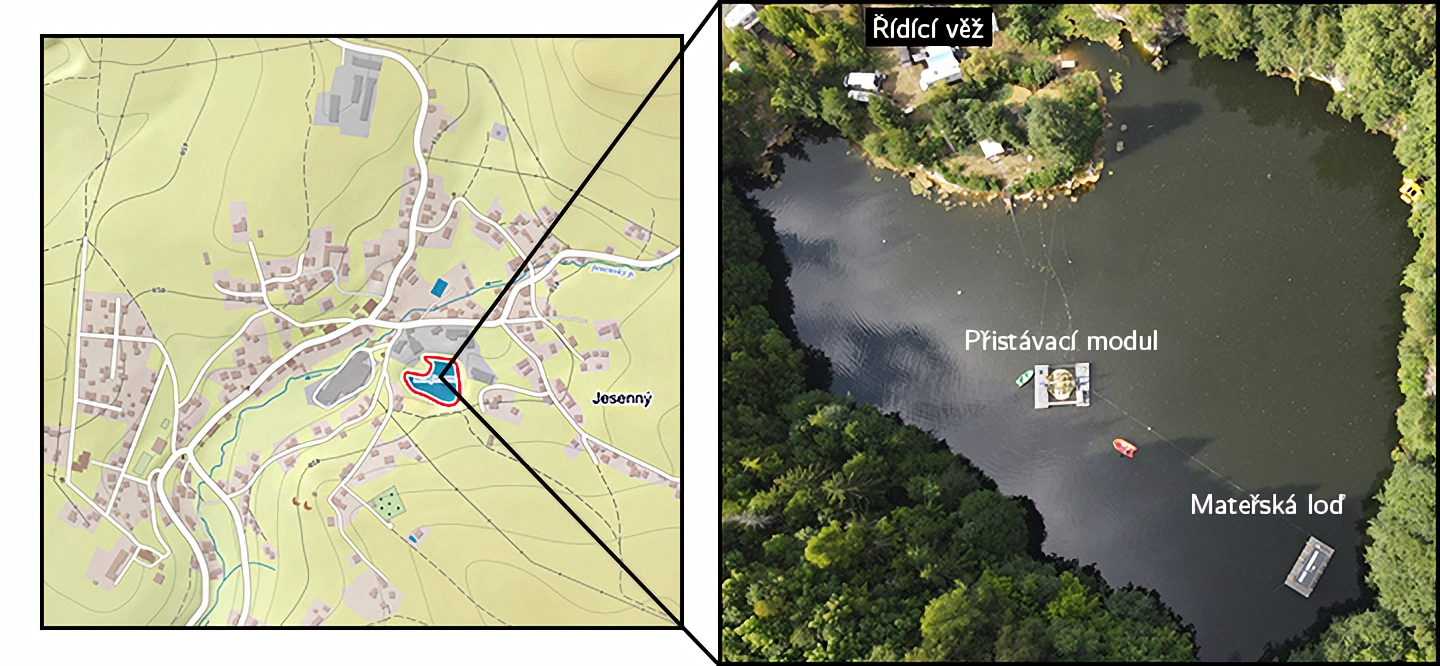
\includegraphics[width=1\linewidth]{figures/map}
        \caption{Detail a lokalita lomu v obci Jesenný (zdroj mapového podkladu: Mapy.cz)}
        \label{fig:map}
    \end{center}
\end{figure}

\subsection{Hlubinná laboratoř H03 DeepLab}
\label{subsubsec:h03_deeplab}
Hydronaut H03 DeepLab je jedinečná výzkumná podvodní laboratoř pro výcvik
posádek v izolovaných, omezených a extrémních podmínkách. Stanice byla zřízena
tak, aby umožnila dlouhodobý pobyt tří členů posádky pod vodní hladinou, přičemž
její konstrukce kombinuje kesonový a ponorkový princip. Díky této unikátní
laboratoří bylo tak umožněno vytvořit podmínky pro dlouhodobý výzkum a sledování
vlivu například tlaku, vlhkosti, stresu, umělého osvětlení a izolovaného
prostředí na člověka nebo použité materiály a vybavení. V rámci mise DIANA plní
roli přistávacího modulu.

\begin{figure}[h]
    \begin{center}
        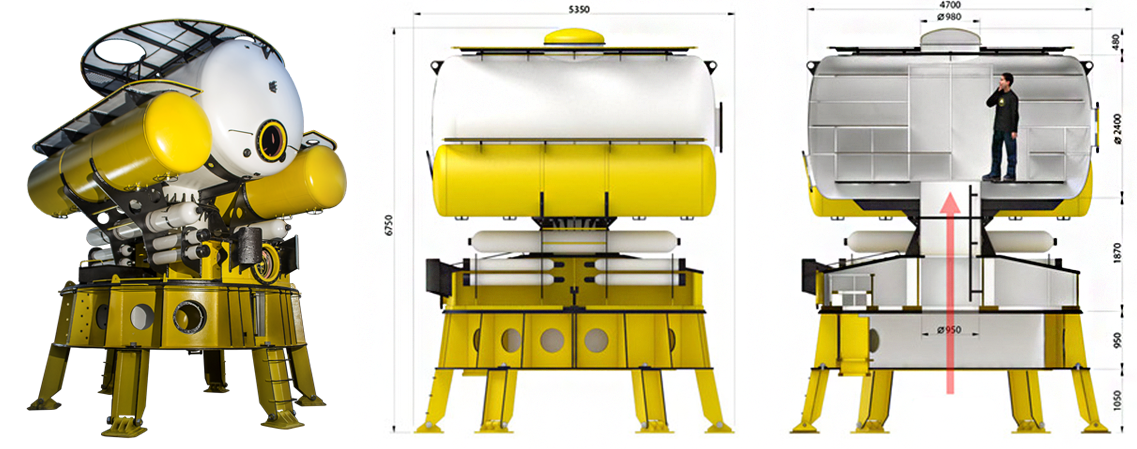
\includegraphics[width=1\linewidth]{figures/habitat}
        \caption{Hlubinná laboratoř H03 DeepLab a její schéma}
        \label{fig:habitat}
    \end{center}
\end{figure}

\subsubsection{Vybavení stanice}
\label{subsubsec:vybaveni_stanice}
Po hardwarové stránce je stanice je vybavena systémy pro monitorování stavu
prostředí uvnitř habitatu a zařízeními pro monitorování fyziologických funkcí
jednotlivých členů posádky. Součástí je také systém pro přenos dat do řídícího
stanoviště.

Pro potřeby například komunikace nebo monitorování fyziologických dat je stanice
vybavena i potřebným softwarem, který je obalen škálovatelným palubním systémem.
Tento systém umožňuje vizualizaci, administraci a hodnocení měřených veličin
(data prostředí, biomedicínská data) společně s obousměrnou komunikaci se všemi
zapojenými účastníky s možností volby různých komunikačních omezení (např. pro
potřeby simulace výpadku komunikace). Vybrané dílčí částí vybavení stanice jsou
detailněji popsány v následujících sekcích.

\subsubsection{Řízení stanice a mise}
\label{subsubsec:rizeni_stanice_mise}
Stanice H03 DeepLab má hlavní komunikační systém zvaný \textit{Common Tongue}.
Ten zajišťuje komunikaci mezi posádkou a podpůrným týmem a umožňuje živé
sledování životních funkcí posádky a vnitřního prostředí. Pomocí tohoto systému
byli subjektům experimentu zadávány úkoly, které jsou sledovány za účelem
vyhodnocení změn chování sledováním vlivu stresu na soustředění a výkonnost
mozku.

\subsubsection{Monitorování atmosféry habitatu}
Jedním z důležitých východisek pobytu v habitatu jsou podmínky prostředí, které
je nezbytné nepřetržitě a spolehlivě monitorovat. Jednou z těchto podmínek je
atmosféra pro jejiž monitorování slouží systém založený na platformě slowRIO
(slow remote IO controller) vyvinutý ve spolupráci s Fakultou strojní (FS ČVUT)
na projektu Hydronaut. Systém monitoruje a poskytuje data prostředí --
mikroklima: absolutní tlak, relativní vlhkost, teplota vzduchu, teplota vody,
čidlo $O_2$, čidlo $CO_2$, čidlo $H_2$, čidlo $CH_4$, intenzita osvětlení, barva
osvětlení a další. Data jsou posílána do palubního počítače.

\subsection{Infrastruktura mise}
\label{subsec:infrastruktura_mise}
Povaha a náročnost stanovených cílů mise se vyžádaly komplexní infrastrukturu
pro podporu celého výzkumného procesu. V této podsekci je uveden stručný přehled
některých součástí infrastruktury včetně harmonogramu mise.

\subsubsection{Harmonogram mise}
\label{subsubsec:harmonogram_mise}
Harmonogram mise byl základním dokumentem, který definoval všechny činnosti v
průběhu mise. Harmonogram byl rozepsaný na úroveň minut pro každého jednotlivého
člena posádky. Ukázku harmonogramu lze vidět na Obr.~\ref{fig:harmonogram}.

\begin{figure}[h]
    \begin{center}
        \begin{framed}
            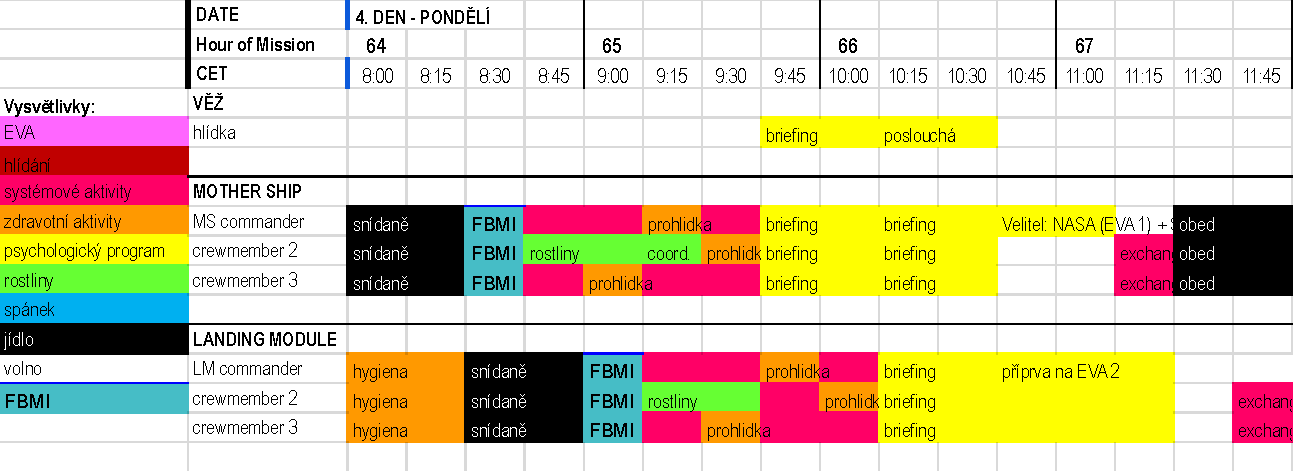
\includegraphics[width=1\linewidth]{figures/harmonogram}
        \end{framed}
        \caption{Ukázka části harmonogramu mise}
        \label{fig:harmonogram}
    \end{center}
\end{figure}

Spolu s harmonogramem byly vytvořeny další dva dokumenty. První z nich byl plán
směn a druhý byl dokument, do kterého se zaznamenávaly všechny významné
události. Plán směn byl vytvořen interně pro každou instituci, jež byla součástí
mise. Každá směna sloužila primárně za účelem monitorování a dokumentace mise.

\subsubsection{Řídicí věž}
\label{subsubsec:ridici_vez}
Řídicí věž hrála v rámci mise DIANA roli stanoviště na Zemi. Komunikovala tedy
se základnou (mateřskou lodí) v souvislosti s prováděním výzkumných a
vzdělávacích programů. Zároveň zde bylo umístěno monitorovací zařízení posádky,
které nepřetržitě sbíralo data a dokumentační a komunikační zařízení.

\begin{figure}[h]
    \begin{center}
        \includegraphics[width=1\linewidth]{figures/monitoring}
        \caption{Monitorování posádky v řídící věži během mise DIANA}
        \label{fig:monitoring}
    \end{center}
\end{figure}

\subsubsection{Povrchová jednotka}
\label{subsubsec:povrchova_jednotka}
Povrchová jednotka byla složena z vedoucího týmu (tři členové stejně jako v
podvodním habitatu), který řídil polohu stanice a systémy podpory života.
Zároveň se povrchová jednotka starala o regulaci specifických parametrů v
závislosti na průběhu mise. Během mise DIANA hrála tato jednotka roli mateřské
lodi, jež sloužila jako stanoviště a kritické zázemí pro velitele posádky. Z
toho místa probíhalo ovládání stanice H03 DeepLab.

\subsection{Neuropsychofyziologická baterie}
\label{subsubsec:neuro_testy}
Neuropsychofyziologická stimulace a diagnostika jedinců byla během mise
realizována prostřednictvím následujících nástrojů:
\begin{enumerate}
    \item \textbf{Kognitivní úlohy v prostředí NEUROP-III} --- posádka opakovaně
          podstoupila náročné diagnostické kognitivní úlohy, zvláště zaměřené na
          sledování exekutivních funkcí primárně v oblasti impulzivního chování,
          riskování, interference nebo inhibice ve smyslu Go-NOGO.
    \item \textbf{Subjektivní hodnocení pomocí NASA TLX} --- jedná se o
          dlouholetý standard pro měření subjektivního vnímání mentální zátěže
          vzhledem ke konkrétním úkolům v pěti dimenzích: mentální náročnost, fyzická
          náročnost, časová náročnost, výkonnost, snaha a frustrace. Posádka byla
          tímto hodnocena během celé mise každý den.
\end{enumerate}

\subsection{Monitorování a měření posádky}
\label{subsec:monitorovani posadky}
Během celého průběhu mise byla posádka neustále monitorována kamerovým systémem
a měřena pomocí validovaných biometrických zařízení, které poskytovaly palubnímu
počítači následující údaje o stavu posádky: tepová frekvence, dechová frekvence,
kožní vodivost. Měření biosignálů je blíže popsáno v další sekci. Zároveň byly
pomocí kamerových záznamů detekovány emoce posádky z výrazů tváře. Na
Obr.~\ref{fig:monitoring} lze vidět snímky z monitorování posádky během mise
DIANA.

\begin{figure}[h]
    \begin{subfigure}[h]{0.48\linewidth}
        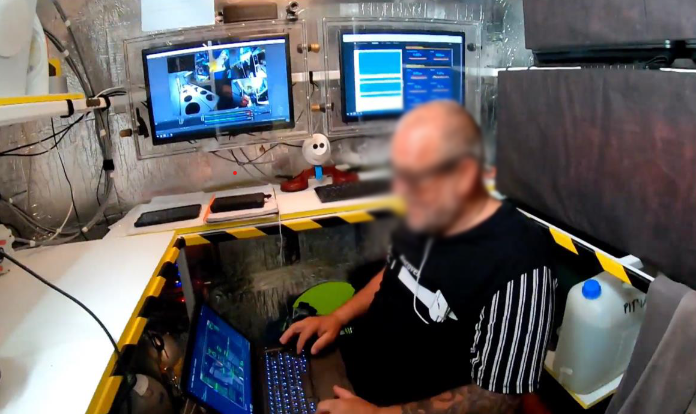
\includegraphics[width=\linewidth]{figures/lander}
        \caption{Snímek z monitorování v přistávacím modulu (interiér modulu)}
    \end{subfigure}
    \hfill
    \begin{subfigure}[h]{0.48\linewidth}
        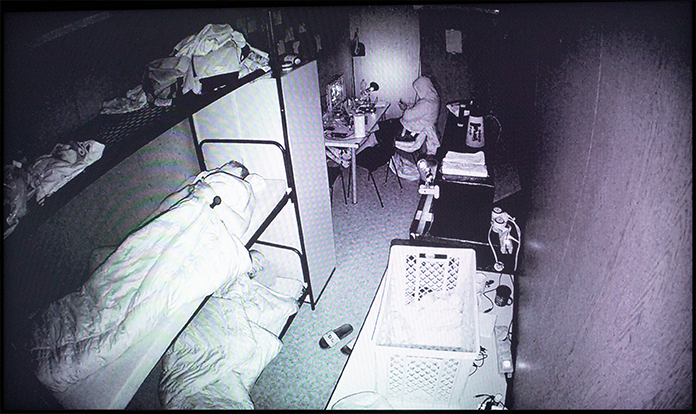
\includegraphics[width=\linewidth]{figures/nightcam}
        \caption{Noční snímek z monitorování posádky mateřské lodi}
    \end{subfigure}
    \caption{Snímky z monitorování posádky během mise DIANA}
\end{figure}

Data z biometrických jednotek byla pomocí bezdrátové síti WLAN (Wi-Fi 2,4 Ghz)
přenášena na datový server a ukládána do InfluxDB. Ostatní kompartmenty mise,
tak mohly živě sledovat fyziologický stav posádky. Díky real-time vizualizaci
bylo také možné dohlížet na správností měření biologických signálů. Předcházelo
se tak situacím jako: nesprávně nalepené či odlepené elektrody, přítomnost
elektromagnetického rušení ovlivňujícího měření nebo výpadky způsobené problémy
s bezdrátovým připojením.

\subsubsection{InfluxDB}
\label{subsec:influx}
InfluxDB\footnote{https://www.influxdata.com} je open-source platforma
poskytující databázi pro časové řady. Zahrnuje rozhraní (API) pro standardní
databázové dotazy. Součástí je i grafické uživatelské rozhraní (GUI) s
modulárními uživatelskými panely pro monitorování dat v reálném čase. Tato
platforma (InfluxDB OSS 2.4) byla využita v rámci mise k uchovávání a
vizualizaci dat.

\subsubsection{Měření biosignálů}
\label{subsubsec:mereni_biosignalu}
V minulé sekci byla zmínka o biometrických datech jako například tepová a
dechová frekvence. Tyto data byla získána pomocí biometrických jednotek, které
však neměří přímo tyto fyziologické indikátory ale biologické signály, konkrétně
srdeční, respirační a elektrodermální aktivitu. Tyto biosignály byly měřeny u
šesti jedinců, konkrétně u posádky mateřské lodi a přistávacího modulu. V
následující sekci je detailněji rozebráno měřící zařízení.

\begin{figure}[h]
    \begin{center}
        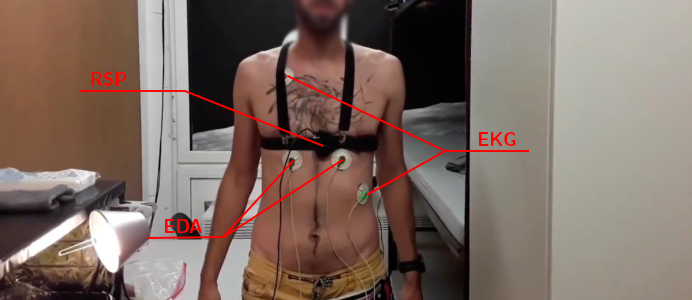
\includegraphics[width=1\linewidth]{figures/sensors}
        \caption{Ukázka měřících čidel na těle člena posádky uvnitř mateřské lodi}
        \label{fig:sensors}
    \end{center}
\end{figure}

\subsubsection{Měřící zařízení}
\label{subsubsec:merici_zarizeni}
Pro měření biosignálu během mise byly použity validované telemedicínské jednotky
\gls{BOREC} (Body recorder), které již dlouhodobě vyvíjíme ve výzkumné skupině
Biomechaniky a asistivních technologií na Fakultě biomedicínského inženýrství
(\gls{FBMI}), ČVUT v Praze. Vzorkovací frekvence zařízení je 250~Hz. Zařízení lze
vidět na Obr.~\ref{fig:borec}.

Respirační aktivita byla měřena pomocí takzvaného dechového pásu, založeného na
tenzometrickém principu. Elektrodermální aktivita byla měřena pomocí dvou
elektrod na hrudi. Toto místo bylo pro potřeby mise vybráno na základě
studie~\cite{Janssen2012}. Elektrická srdeční aktivita byla měřena využitím
jednosvodového systému, přičemž byl svod zaznamenáván v konfiguraci II. Jednotka
včetně snímačů biosignálů také obsahuje tlakové a gyroakcelometrické senzory.

Bezdrátové připojení jednotek je zajištěno díky standardu IEEE 802.11 (Wi-Fi
2,4~GHz). Komunikační protokol mezi zařízením a klientem na straně počítače je
Modbus TCP~\cite{modbus}, který umožňuje přistup k senzorům jednotky a stažení
dat z cyklických redundantních vyrovnávacích pamětí. Každá jednotka má svou
vlastní jedinečnou MAC adresu a očekává adresu IP od serveru DHCP. Klient na PC
má přístup ke všem snímačům místní sítě.

\begin{figure}[h]
    \begin{center}
        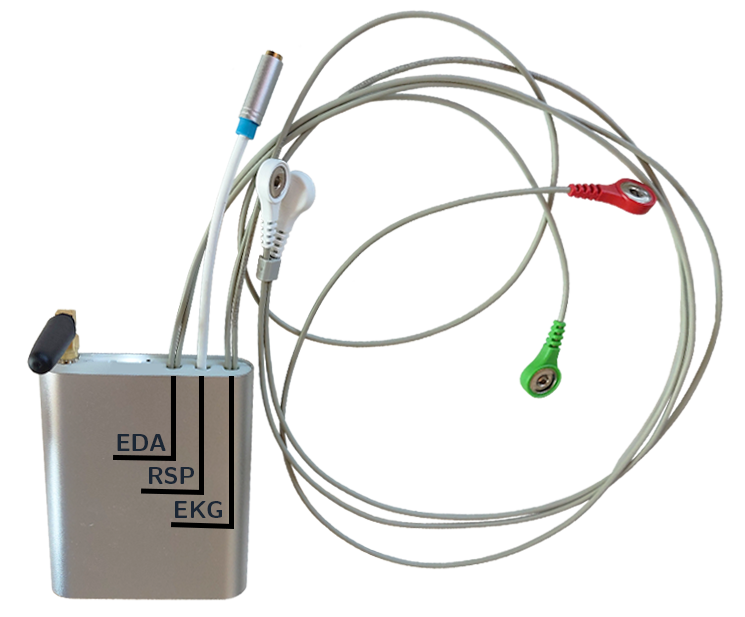
\includegraphics[width=0.65\linewidth]{figures/borec}
        \caption{Telemedicínská jednotka \gls{BOREC} použita během mise}
        \label{fig:borec}
    \end{center}
\end{figure}


\subsection{Studie}
\label{subsec:studie}
%!#TODO: Doplnit referenci na prilohu s informovanym souhlasem
Měření dat probíhalo pod Filozofickou fakultou Univerzity Palackého v Olomouci
(\gls{FF UPOL}). Všichni probandi poskytli informované souhlasy pro část
diagnostickou i pro samotný experiment (viz Příloha~\ref{}). Informované
souhlasy umožňují anonymizované využití dat. Získání dat pod FF UPOL probíhalo
podle etického metakodexu Evropské federace psychologických asociací
(\gls{EFPA}). Informované souhlasy jsou i ke všem nahrávkám obrazových dat a
rozhovorů členů posádky. Bezpečí participantů bylo jištěno v několika
technických rovinách prostřednictvím hlavního řešitele \textit{1st Cloud
Republic a.s.} projektu TL05000228.

\section{Použité datasety}
\label{sec:datasety}
Pro účely diplomové práce bylo použito několik veřejně dostupných datasetů
včetně dat z mise DIANA. V následujících sekcích jsou stručně rozebrány
jednotlivé datasety, přičemž první dva sloužily primárně pro účely detekce
kognitivní zátěže.
\subsection{WESAD}
\label{subsec:wesad}
Dataset WESAD~\cite{wesadDataset} (\textit{Wearable Stress and Affect
Detection}) je multimodální dataset navržený pro výzkum v oblasti hodnocení
stresu a emocí za použití nositelných senzorů. Tento dataset byl vytvořen s
cílem přispět k vývoji pokročilých algoritmů strojového učení pro analýzu
fyziologických signálů a rozpoznání emocí. WESAD obsahuje data získaná od 15
účastníků, přičemž každý z nich prošel sérií experimentů v laboratorních
podmínkách.

Data byla v datasetu získána ze dvou nositelných zařízení. Prvním zařízením byl
\textit{RespiBAN}\footnote{Zařízení \textit{RespiBAN} již není vyráběno},
nositelný senzor umístěný na hrudi se vzorkovací frekvencí 700~Hz, který
zaznamenával elektrokardiogram, elektrodermální aktivitu, elektromyogram,
respirační signál a teplotu těla. Druhé zařízení byl chytrý náramek
\textit{Empatica E4}\footnote{\url{https://www.empatica.com/research/e4}}, který
zaznamenává krevní tlak (64~Hz), elektrodermální aktivitu (4~Hz), teplotu těla
(4~Hz) a tříosou akceleraci (32~Hz). Experiment, který byl proveden pro sběr
dat, zahrnoval celkem čtyři fáze:
\begin{enumerate}
    \item \textbf{Základní úroveň (Baseline condition)} --- účastník byl požádán, aby
    seděl/stál v klidu po dobu 20 minut.
    \item  \textbf{Stresový úkol (Stress condition)} --- účastník musel pět minut
    přednášet před publikem a poté vyřešit matematický úkol, který byl navržen
    tak, aby vyvolal stres.
    \item  \textbf{Relaxační úkol (Amusement condition)} --- účastník sledoval
    komediální video, které mělo vyvolat příjemné emoce.
    \item  \textbf{Řízená meditace (Meditation)} --- účastník prováděl řízenou
    meditaci, jejíž cílem bylo navození do stavu blízkého neutrálnímu
    afektivnímu stavu.
\end{enumerate}

WESAD poskytuje časově synchronizovaná, předzpracovaná a anotovaná data z těchto
nositelných senzorů. Pro účely diplomové práce byly použity signály ze zařízení
\textit{RespiBAN}, konkrétně srdeční, respirační a elektrodermální aktivita. Pro
úlohy hodnocení kognitivní zátěže byla základní úroveň označena jako klidový stav
a stresové úkoly byly označeny jako stav kognitivní zátěže.

\subsection{CLAS}
\label{subsec:clas}
Dataset CLAS~\cite{clasDataset} (\textit{Cognitive Load, Affect, and Stress
Recognition}) je podobně jako WESAD multimodální dataset vytvořený pro výzkum v
oblasti rozpoznávání kognitivní zátěže a emocí za použití nositelných senzorů a
dalších datových zdrojů. Dataset zahrnuje data získaná od 62 účastníků, kteří
byli vystaveni různým úkolům a podnětům navrženým tak, aby vyvolaly různé úrovně
kognitivní zátěže a emocí. Mezi tyto podněty patřily například matematické úlohy
nebo Stroopův test. Každý účastník byl zároveň měřen i v klidu (dataset stav
označuje jako Baseline). Během přechodů mezi jednotlivými úkoly bylo účastníkům
puštěno neutrální video nebo byl účastník požádán, aby vyplnil dotazník (dataset
označuje jako Neutral). 

Fyziologická data v rámci tohoto datasetu byla měřena zařízením
\textit{Shimmer3}\footnote{\url{https://shimmersensing.com}} se vzorkovací
frekvencí 256~Hz. Mezi měřené biologické signály patří elektrokardiogram,
elektrodermální aktivita a fotopletysmogram. Pro úlohy hodnocení kognitivní
zátěže byl Baseline stav označen jako klidový stav a stresové úkoly byly
označeny jako stav kognitivní zátěže. 

\subsection{Data z vesmírné analogové mise DIANA}
\label{subsec:data_diana}
Pro potřeby diplomové práce poskytla \gls{FF UPOL} data z vesmírné analogové
mise DIANA. Součástí dat jsou osmidenní 24 hodinové záznamy biologických
signálů, kamerových záznamů a anotace v podobě časů kognitivních úloh pro
každého člena posádek. Využitými signály v této práci jsou elektrokardiogram
spolu s elektrodermální a respirační aktivitou.

\section{Zpracování biosignálů}
\label{sec:zpracovani_biosignalu}
Důležitým krokem při analýze biosignálů je jejich zpracování. V této sekci jsou
popsány použité algoritmy, které byly implementovány v programovacím jazyce
Python, využitím knihovny \textit{Neurokit2} (viz sekce~\ref{subsec:neurokit}).
\subsection{Zpracování elektrické srdeční aktivity}
\label{subsec:zpracovani_ekg}
Pro zpracování EKG záznamů byla implementována metoda podle Kalidase a
Tamila~\cite{kalidas2017}, která je založena na stacionární vlnkové transformaci
(\gls{SWT}). Metoda vychází z populárního Pan-Tompkinsova~\cite{Tompkins1985}
algoritmu, nicméně pro odstranění šumu a zvýraznění QRS komplexů používá
\gls{SWT} namísto pásmové propusti. Stacionární vlnková transformace je metoda
rozkladu signálu na jednotlivá frekvenční pásma pomocí mateřské
vlnky~\cite{Nason1995}. Metoda byla zvolena na základě následující
sekce~\ref{subsubsec:vyberqrs}.

\begin{figure}[H]
    \begin{center}
        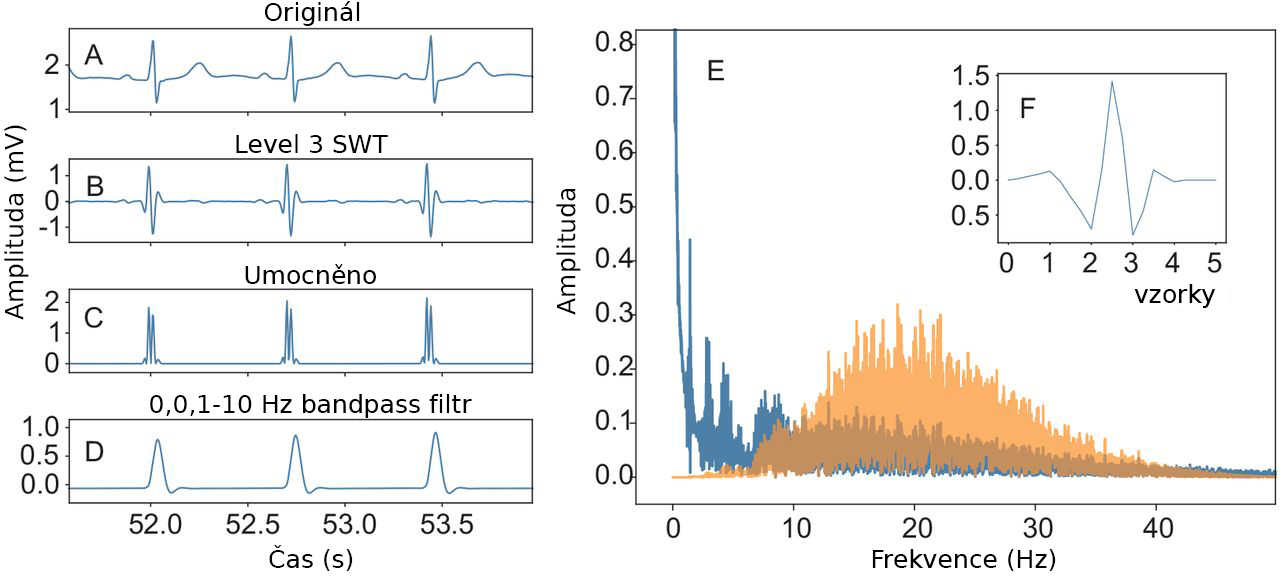
\includegraphics[width=1\linewidth]{figures/kalidas2017}
        \caption{\textbf{A-D)} Kroky zpracování EKG pro algoritmus podle
            Kalidase a Tamila~\cite{kalidas2017} \textbf{E)} Frekvenční spektrum
            nefiltrovaného EKG se vzorkovací frekvencí 250~\si\Hz~(modrá) a EKG po
            SWT 3. řádu (oranžová). \textbf{F)} vlnka rodiny Daubechies 3. řádu.
            (Upraveno a převzato z~\cite{Porr2019})}
        \label{fig:kalidas_processing}
    \end{center}
\end{figure}

V tomto algoritmu se stacionární vlnková transformace provádí na EKG signálu
využitím vlnky rodiny Daubechies třetího řádu. Po provedení \gls{SWT} se
extrahují koeficienty, které se následně umocní. Následně je využito filtrace
pásmovou propustí (Butterworthův filtr) ke zvýšení citlivosti a přesnosti
detekce. Postup detekce R vln na filtrovaném signálu je pak totožná s detekcí
Pan-Tompkinsova algoritmu~\cite{Tompkins1985}. Jednotlivé části zpracování lze
vidět na Obr.~\ref{fig:kalidas_processing}.

\subsubsection{Metodika výběru QRS detektoru}
\label{subsubsec:vyberqrs}
Vzhledem k tomu, že neexistuje žádný jednotný standard či systematický postup
pro zpracování EKG a výběr \enquote{správného} QRS detektoru pro určitou
aplikaci, bylo v rámci této práce realizováno statistické porovnání populárních
algoritmů. Měřítko přesnosti QRS detekce algoritmu vycházelo z výpočtu absolutní
vzdálenosti od původní \enquote{skutečné} polohy R vlny. Pro benchmarking
detektorů byly použity následující anotované datasety:

\begin{table}[h]
    % \footnotesize
    \begin{center}
        \caption{\label{tab:bench_datasets} Vybrané datasety pro benchmarking
            QRS detektorů z PhysioNetu~\cite{PhysioNet}}
        \renewcommand{\arraystretch}{1.3}
        \begin{tabular}{p{12cm}c}
            \toprule
            \textbf{Dataset}                                                                                                 & \textbf{Probandi} \\ \midrule
            MIT-BIH Arrhythmia Database~\cite{MITBIHArrhythmia}                                                              & 48                \\
            MIT-BIH Normal Sinus Rhythm Database~\cite{Beth1990}                                                             & 18                \\
            Glasgow University Database~\cite{GUDB}                                                                          & 25                \\
            Fantasia Database~\cite{FANTASIA}                                                                                & 40                \\
            Lobachevsky University Electrocardiography Database~\cite{LUDB}                                                  & 200               \\
            Simultaneous physiological measurements with five devices at different cognitive and physical loads~\cite{IFADO} & 13                \\
            Pulse Transit Time PPG Dataset~\cite{USYD}                                                                       & 22                \\
            \bottomrule
        \end{tabular}
    \end{center}
\end{table}

Za účelem zjištění adaptability byly vybrány různorodé datasety algoritmu. Pro
statistické zpracování bylo využito lineárních smíšených modelů (\gls{LMM}).
Použité statistické metody jsou podrobněji popsány v
kapitole~\ref{sec:statisticke_metody}. Pro srovnání metod byl v programovacím
jazyce R vytvořen následující statistický model:
\begin{equation}
    \text{Skóre} = \beta_0 + \beta_1\text{Metoda} + u_{\text{Dataset}} + u_{\text{Participant}} + \epsilon
\end{equation}
který specifikuje lineární smíšený model pomocí funkce \texttt{lmer} z balíku
\texttt{lme4}\footnote{\url{https://github.com/lme4/lme4}}. Model byl použit k
predikci závislé proměnné Skóre na fixním efektu $Metoda$ a dvou náhodných
efektech: $Dataset$ a $Participant$. Dále problematice této sekce není věnována
pozornost, jelikož není předmětem této práce. 

\subsection{Zpracování respirační aktivity}
\label{subsec:zpracovani_rsp}
Pro zpracování respirační aktivity byl implementován
algoritmus~\cite{Khodadad2018}, který je založen na průchodech nulou (\gls{ZC},
Zero-Crossing). Originální signál je nejdříve filtrován pásmovou propustí
0,05--3~Hz pro odstranění stejnosměrné složky a vyšších nežádoucích frekvencí
tak, aby bylo možné spolehlivě detekovat \gls{ZC}. Tím jsou zachovány dechové
frekvence menší než tři a vyšší než 180 dechů za minutu. Následně jsou
detekovány indexy náběžných a sestupných průchodů nulou, mezi kterými došlo k
hledání lokálních extrémů.

\begin{figure}[h]
    \begin{center}
        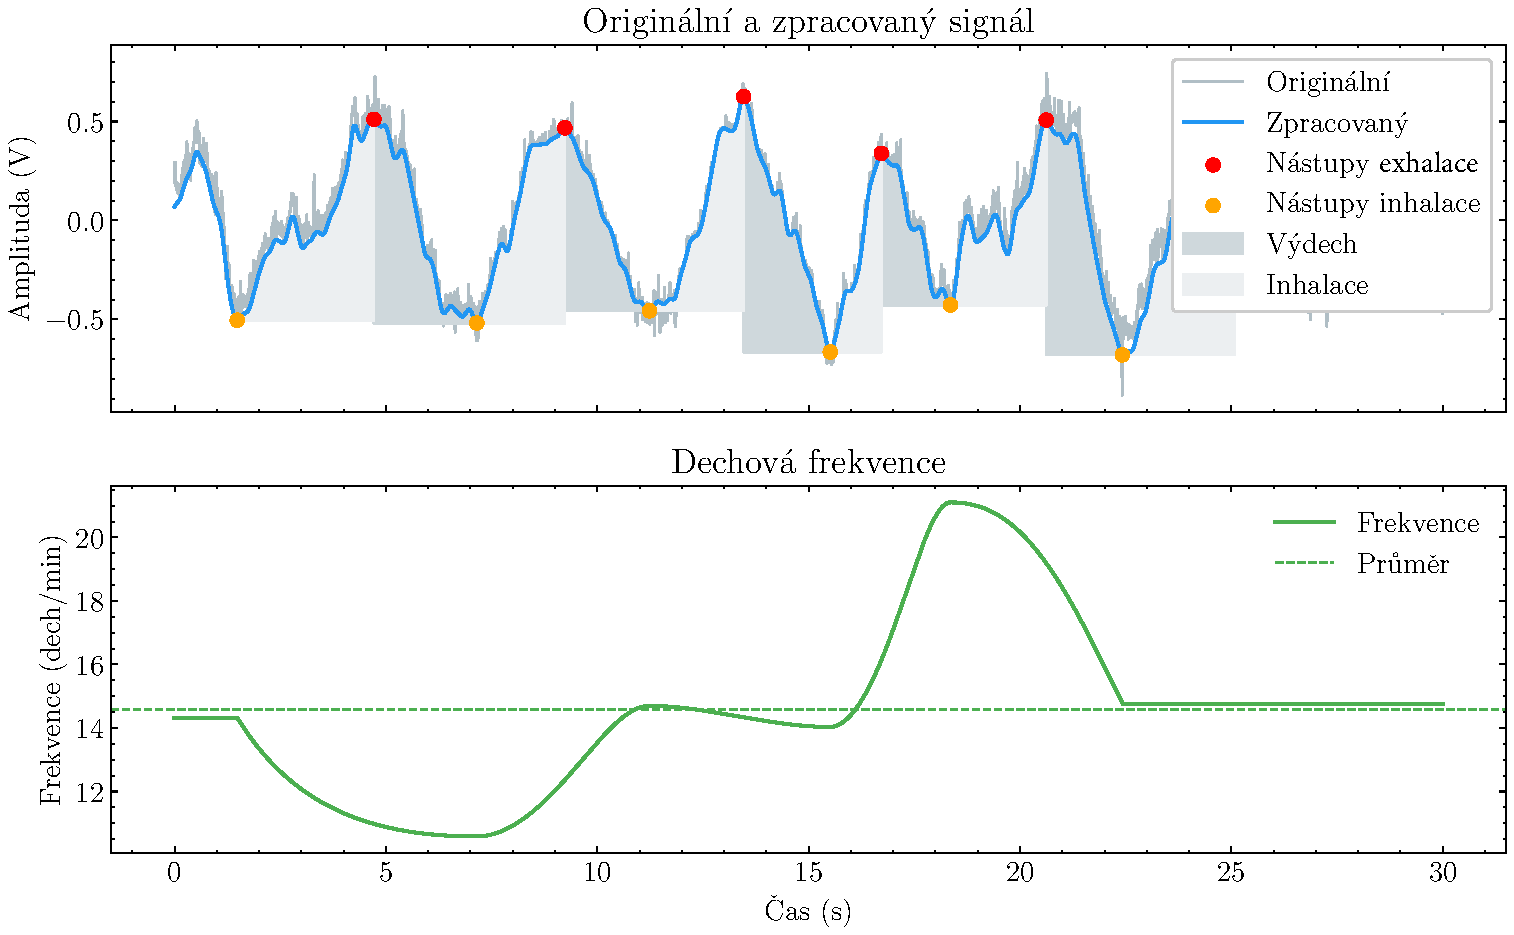
\includegraphics[width=1\linewidth]{figures/rsp_test}
        \caption{Příklad zpracování RSP pomocí implementované metody}
        \label{fig:rsp_test}
    \end{center}
\end{figure}

Zachovány jsou ve výsledku pouze ty extrémy, které mají minimální vertikální
vzdálenost od svého přímého souseda, tudíž kritérium pro detekci odlehlých
hodnot bylo definováno v absolutním rozdílu amplitud mezi sousedními extrémy. V
rámci dechové frekvence jsou mezi jednotlivými nádechy interpolovány data
využita monotónní kubické interpolace. Aplikace metody na reálném signálu lze
vidět na Obrázku~\ref{fig:rsp_test}.

\subsection{Zpracování elektrodermální aktivity}
\label{subsec:zpracovani_eda}
Zpracování elektrodermální aktivity vychází z metod~\cite{vanhalem2020}
a~\cite{posada2016}. Signál je nejdříve filtrován Butterworthovou horní propustí
4. řádu s mezní frekvencí 3~\si\Hz. Následně je ze signálu extrahována fázická a
tonická složka pomocí dolní a horní propusti o mezních frekvencích 0,05~\si\Hz.

\begin{figure}[h]
    \begin{center}
        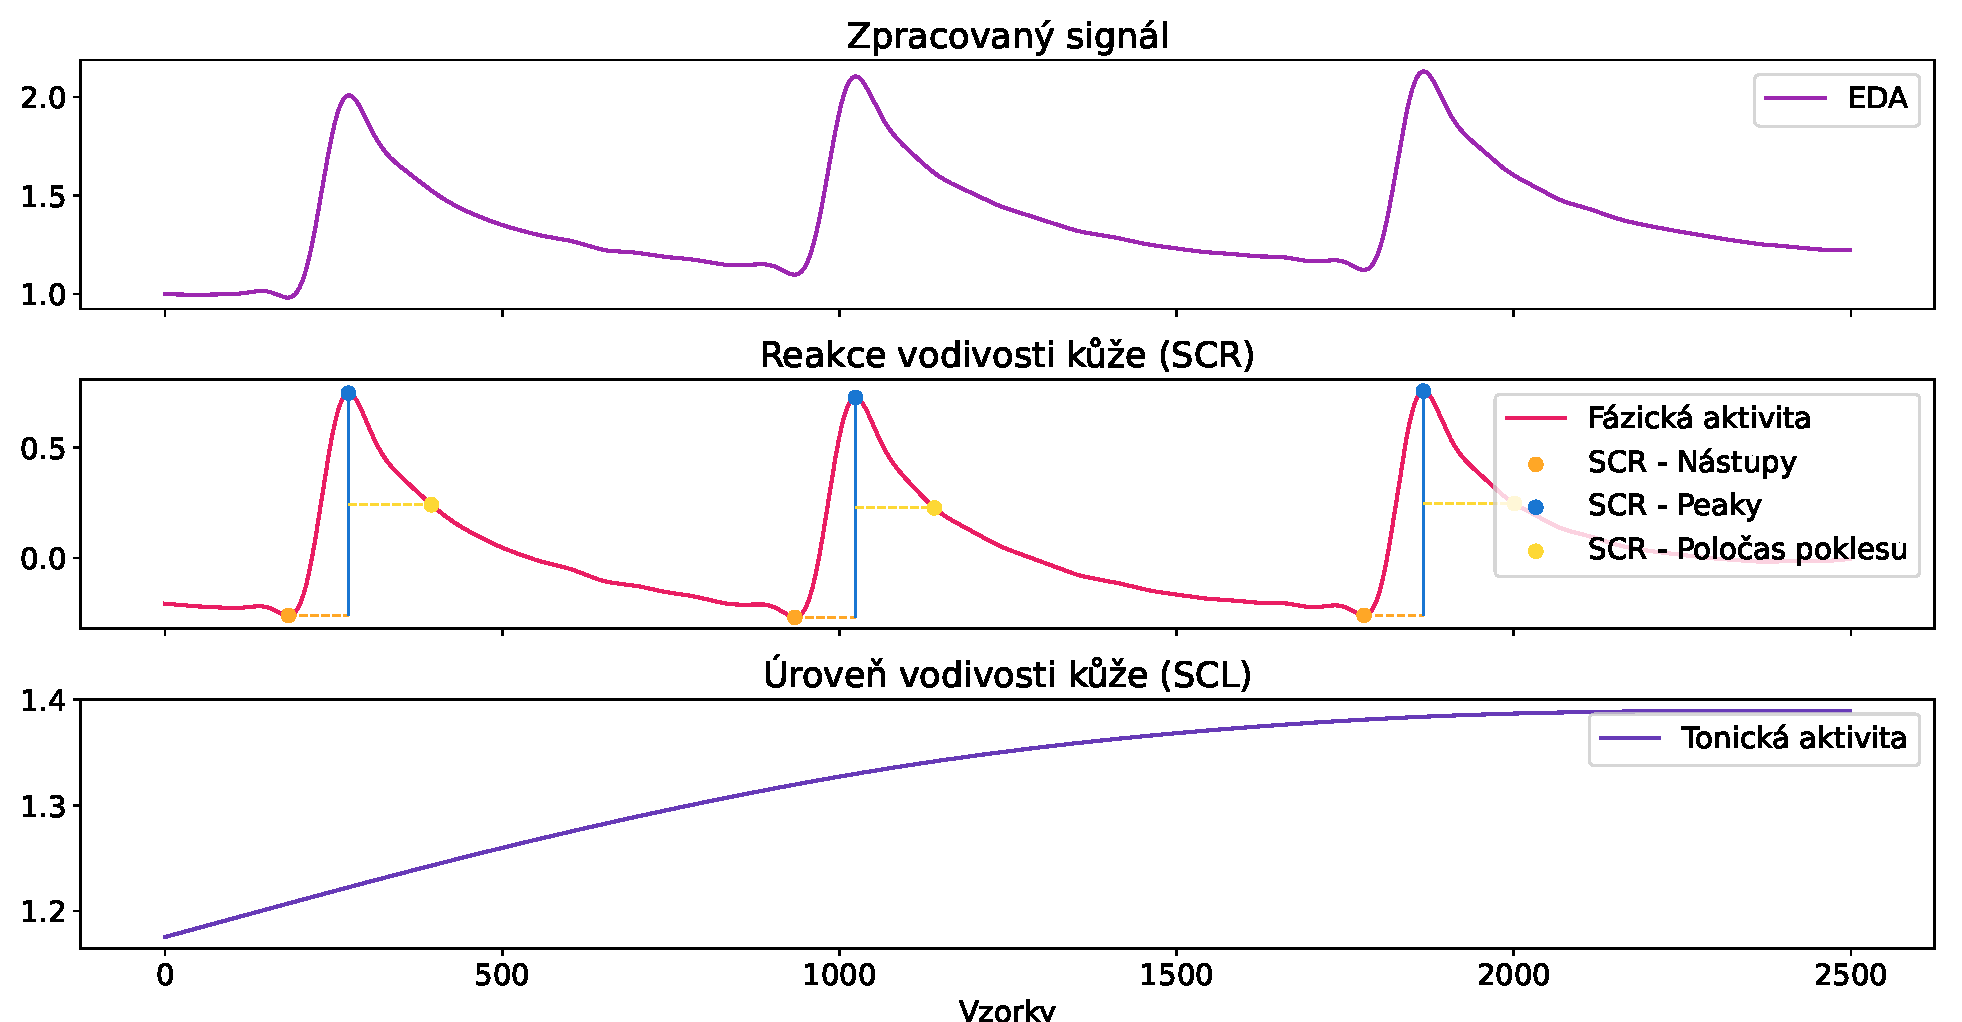
\includegraphics[width=1\linewidth]{figures/eda_test}
        \caption{Příklad zpracování EDA pomocí implementovaných metod}
        \label{fig:eda_test}
    \end{center}
\end{figure}

Dále byl použit Savitzky-Golayův frekvenčně neselektivní filtr k dalšímu
vyhlazení fázické složky za účelem hledání \gls{SCR} vrcholků. K detekci
vrcholků byla využita funkce \texttt{find\_peaks()} z knihovny
Scipy\footnote{\url{https://docs.scipy.org}}. Kritérium pro detekci vrcholků
bylo definováno jako monotónní nárůst o 0,5s následovaný stejným poklesem.
Výsledek aplikované metody lze vidět na Obrázku~\ref{fig:eda_test}.

\subsection*{Neurokit}
\label{subsec:neurokit}
Knihovna \textit{Neurokit2}, na jejíž vývoji se
podílím\footnote{\url{https://neuropsychology.github.io/NeuroKit/authors.html}},
poskytuje pokročilé metody pro zpracování a vizualizaci biosignálu. Jednotlivé
metody zároveň nabízejí možnost si vybrat z mnoha implementovaných algoritmů. V
této práci byla knihovna použita pro zpracování respirační, elektrodermální a
elektrické srdeční aktivity včetně zpracování a výpočtu \gls{HRV} parametrů.


\section{Zpracování a analýza dat z mise DIANA}
V následující sekci je popsána metodika zpracování a analýzy dat z vesmírné
analogové mise DIANA. Data z mise byla poskytnuta v podobě komprimovaného
záložního souboru obsahující snímek databáze InfluxDB (viz
sekce~\ref{subsec:influx}). Tento snímek byl použit pro obnovu databáze, která
obsahovala veškeré data s časovými značkami. Pro export a práci s daty byla
využita Python knihovna
\textit{InfluxDB-Python}\footnote{https://github.com/influxdata/influxdb-python},
jež poskytuje rozhraní mezi InfluxDB a programovacím jazykem Python. 
\label{sec:zpracovani_dat_diana}
\subsection{Zpracování exportovaných segmentů biosignálů}
\label{subsec:prezpracovani_segmentu}
Pro každého člena posádky byly exportovány segmenty biosignálů o délce 30s s
50\% překryvem na základě poznatků
v~\cite{Castaldo2019,Kim2021,Pecchia2018,Shaffer2020,Tervonen2021}. Zpracování
biosignálu vycházelo z metodiky popsané v sekci~\ref{sec:zpracovani_biosignalu}.
U každého segmentu proběhlo hodnocení jeho kvality podle dvou kritérií:
\begin{itemize}
    \item Hodnocení kvality \gls{EKG} signálu pomocí heuristické fúze a fuzzy
    komplexního hodnocení podle~\cite{Zhao2018}.
    \item Hodnocení detekovaných R vln z hlediska časové kontroly náhlých
    nefyziologických změn v po sobě jdoucích R-R intervalech.
\end{itemize}
Segmenty které vykazovali nežádoucí anomálie v rámci hodnotících kritérií byly
vyřazeny. Ze segmentů bylo dále vypočteno následně přes 100 různých parametrů
pro účely analýzy dat. Mezi tyto parametry patřily například běžné statistické
charakteristiky (průměr, medián, směrodatná odchylka a další) nebo nelineární a
časové \gls{HRV} parametry. Zpracované segmenty byly zároveň anotovány, a to z
hlediska spánkového cyklu. Dále byly identifikovány a označeny v časech
kognitivních testů. Z časových důvodu nebyly pro účely této práce ostatní
aktivity během mise anotovány, i přes dostupnost kamerových záznamů. Seznam
všech počítaných parametrů je součástí přílohy v souboru
\texttt{all\_params.csv}.

\subsection{Čistění dat}
\label{subsec:cisteni_dat}
Ze souborů vypočtených parametrů byly vynechány všechny parametry, jejichž
sloupce obsahovali \texttt{NaN} hodnoty. Dále byly parametry korelovány a
odstranili se ty, které byly vzájemně dokonale korelované ($|r| > 0,999$). Poté
se odstranili odlehlé hodnoty na základě absolutní odchylky mediánu od mediánu.

\subsection{Sledované veličiny}
\label{subsec:sledovane_veliciny}
Pro účely analýzy \gls{NPF} adaptace probandů v průběhu mise byly vybrány a
sledovány především následující \gls{HRV} parametry:

\subsection{Tvorba hypotetických LMM modelů}
\label{subsec:tvorba_modelů}



\section{Explorační analýza a předzpracování datasetů}
\label{sec:exploracni_analyza}
V této sekci je rozebrán proces zpracování a zkoumání souborů dat, konkrétně
datasetů CLAS a WESAD, jehož cílem bylo identifikovat vzorce, vztahy a trendy,
které nemusí být okamžitě zřejmé. Cílem explorační analýzy bylo získat poznatky
a vytvořit hypotézy o datech, které napomáhali při tvorbě paradigmatu detekce \gls{CL}.
\subsection{Předzpracování datasetů}
\label{subsec:predzpracovani_datasetu}
Z datasetů byly extrahovány potřebné biosignály, které byly následně zpracovány
a normalizovány na úrovní subjektů. Metodika zpracování vychází ze
sekce~\ref{sec:zpracovani_biosignalu}. Normalizace byla provedena škálováním
biosignálů tak, aby měly průměrnou hodnotu nula a směrodatnou odchylku jedna. To
bylo dosaženo odečtením střední hodnoty biosignálu od každé jeho hodnoty a
následným vydělením směrodatnou odchylkou.

Vzhledem k tomu, že dataset CLAS neobsahuje signál RSP, byl tento signál
vytvořen pomocí metody \gls{EDR} (ECG-Derived Respiration). Jedná se o extrakci
informace o dýchání z elektrokardiogramu. Knihovna \textit{Neurokit2} poskytuje
implementaci algoritmu podle~\cite{VanGent2019}, jež byla pro tyto účely
použita.

Následně byly všechny signály segmentovány na 5s, 5s s 50\% překryvem a 1s
úseky. Z těchto segmentů byly poté vytvořeny příznaky pro účely strojového
učení. Blíže je tvorba těchto příznaků a jejich využití popsáno v
sekci~\ref{sec:hybridni_detekce}. Byly ponechány pouze ty segmenty, které svojí
třídou korespondovaly žádanému kognitivnímu stavu.

\begin{figure}[h]
    \centering
    \framebox[\textwidth]{%
        \begin{subfigure}[b]{0.45\textwidth}
            \dirtree{%
                .1 Datasets.
                .2 WESAD.
                .3 S2.
                .4 S2.pkl.
                .4 $\vdots$.
                .3 S3.
                .3 $\vdots$.
                .2 CLAS.
                .3 Part1.
                .4 full\_ecg.csv.
                .4 full\_gsr\_ppg.csv.
                .4 $\vdots$.
                .3 Part2.
                .3 $\vdots$.
            }
            \caption{Původní struktura datasetů}
            \label{subfig:tree1}
        \end{subfigure}
        \hfill
        \begin{subfigure}[b]{0.45\textwidth}
            \dirtree{%
                .1 Datasets.
                .2 WESAD.
                .3 merged\_1s.pkl.
                .3 merged\_5s.pkl.
                .3 merged\_5s\_2s.pkl.
                .3 $\vdots$.
                .2 CLAS.
                .3 merged\_1s.pkl.
                .3 merged\_5s.pkl.
                .3 merged\_5s\_2s.pkl.
                .3 $\vdots$.
            }
            \caption{Zpracované datasety}
            \label{subfig:tree2}
        \end{subfigure}
    }
    \caption{Porovnání struktury původních a zpracovaných datasetů}
    \label{fig:struktura_datasetu}
\end{figure}

\subsection{Explorace dat}
\label{subsec:explorace_dat}
Oba datasety byly po předzpracování zkoumány pomocí nástrojů knihovny
\textit{Pandas} v programovacích jazyce Python. Datasety tak byly popsány
například základními statistickými údaji, kde byla brána primárně zřetel na
rozdělení tříd. Na Obr.~\ref{fig:rozdeleni_trid} lze tak vidět, že oba datasety
vykazují výraznou nevyváženost tříd. Dále byly korelovány jednotlivé signály
datasetů, bylo nahlíženo na jejich distribuce, a byly vyšetřeny případné záporné
nebo neplatné hodnot. Tato šetření byla provedena i na individuální úrovni. Celý
postup s vizualizovanými výsledky se nachází v datové příloze, v podobě
interaktivního prostředí Jupyter Notebook\footnote{\url{https://jupyter.org}} s
názvem souboru \texttt{exploratory\_analysis\_example}.

\begin{figure}[h]
    \begin{subfigure}[h]{0.48\linewidth}
        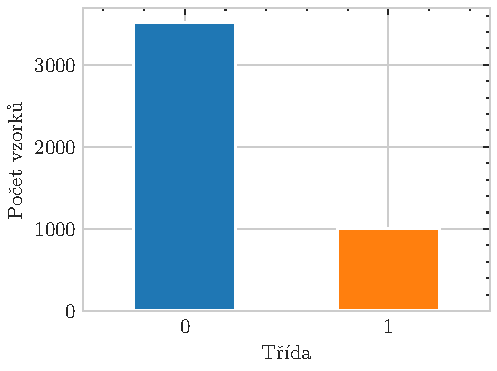
\includegraphics[width=\linewidth]{figures/wesad_labels}
        \caption{Rozdělení datasetu WESAD}
    \end{subfigure}
    \hfill
    \begin{subfigure}[h]{0.48\linewidth}
        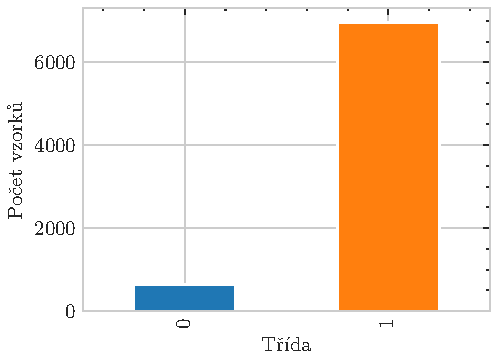
\includegraphics[width=\linewidth]{figures/clas_labels}
        \caption{Rozdělení datasetu CLAS}
    \end{subfigure}
    \caption{Srovnání rozdělení tříd vybraných datasetů. Třída 0 vyjadřuje
    klidový stav a třída 1 vyjadřuje kognitivní zátěž.}
    \label{fig:rozdeleni_trid}
\end{figure}

Během explorace dat byla také zkoumána separovatelnost dat v
nízkodimenzionálních prostorech použitím techniky \gls{UMAP}~\cite{umap2018}
(Uniform Manifold Approximation and Projection) právě pro redukci
dimenzionality. Cílem bylo vizualizovat soubor dat ve formě nižších dimenzí k
získání přehledu o rozdělení tříd a nadhled nad smyslem a rozpoložení dat.
Výsledky této vizualizace je možné vidět na Obr.~\ref{fig:umap}, kde jsou
oranžově vyznačeny body, jež odpovídají kognitivní zátěži.

\begin{figure}[h]
    \begin{subfigure}[h]{0.48\linewidth}
        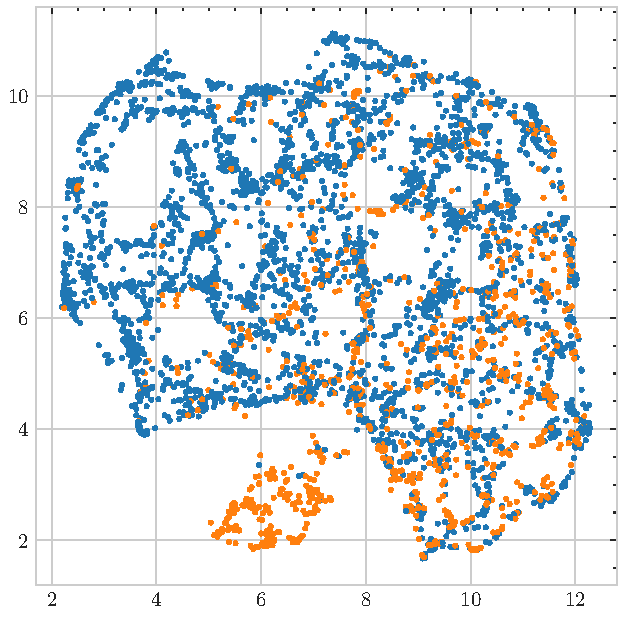
\includegraphics[width=\linewidth]{figures/wesad_umap}
        \caption{WESAD}
    \end{subfigure}
    \hfill
    \begin{subfigure}[h]{0.48\linewidth}
        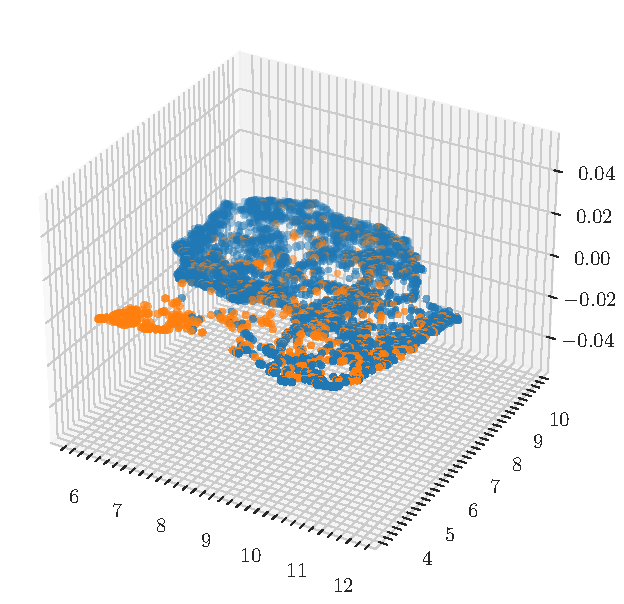
\includegraphics[width=\linewidth]{figures/clas_umap}
        \caption{CLAS}
    \end{subfigure}
    \caption{Vizualizace UMAP projekcí extrahovaných příznaků z datasetu WESAD
    do 2D (vlevo) a 3D latentního prostoru (vpravo). Oranžově třída 1 a modře
    třída 0}
    \label{fig:umap}
\end{figure}

V metodě bylo využito Euklidovské vzdálenostní metriky s hodnotou 0,1 a počtem
sousedních bodů 15. Tyto nízké hodnoty byly zvoleny pro účely zachycení lokální
struktury dat (potenciálně na úkor celkového obrazu), jak ukazuje
Obr.~\ref{fig:umap}. Výsledek 3D projekcí naznačuje potencionální lineární
separovatelnost u malé části souboru. U zbytku souboru by bylo oddělení
pravděpodobně zřetelnější ve vyšších dimenzích a možná nebude lineární. V úvahu
tak přichází strojové učení.

\section{Detekce CL využitím vícerozměrných časoprostorových kauzálních vzorů}
\label{sec:hybridni_detekce}
V této podkapitole je popsán postup realizace nového multimodálního přístupu pro
detekci kognitivní zátěže pomocí periferních biosignálů (\gls{EKG}, \gls{RSP},
\gls{EDA}), které bylo vytvořeného v rámci této diplomové práce.
\subsection{Formulace problému}
\label{subsec:definice_problemu}
V předešlé sekci byl popsán proces předzpracování dat, jehož výsledkem je nová
multidimenzionální množina segmentovaných fyziologických signálů $\mathcal{F}$.
Dimenze této množiny je rovna počtu snímaných signálů, lze tedy dál hovořit jako
o kanálech $c$. Vybraný segment z kanálu $c$ reprezentuje časovou řadu, jejiž
každý vzorek je zachycen v určitém čase $t$, a představuje průběh fyziologické
události (\gls{NPF} událost).

V rámci jednotlivých pozorovaných fyziologických událostí $X^i$, lze modelovat
časově kauzální vztahy, které lze díky Grangerově kauzalitě (viz
sekce~\ref{subsec:granger}) matematicky popsat unikátním orientovaným grafem
$G=(V,E)$ -- definovanou uspořádanou množinou vrcholů a hran. Tím je umožněno
temporální kódování specifického příčinného kognitivního stavu pro konkrétní
segment vybraného kanálu $c$. Nelze však předpokládat, že je tak zachycena
veškerá komplexní dynamika, která je ve biosignálech přítomna, včetně toho, že
nemusí být plně zachyceny interakce napříč kanály $c$.

Tento problém je kompenzován použitím vícerozměrných časoprostorových vzorů
(\gls{GAF}, Gramian Angular Fields) odvozených z Gramových matic. Tyto vzory
zachycují určitý druh temporální i prostorové korelace v rámci fyziologických
událostí. V následujících sekcích je dále popsána tvorba zmíněných příznaků
společně s jejich aplikací v rámci strojového učení.

\subsection{Tvorba kauzálních vícerozměrných matic}
\label{subsec:kauzalni_matice}
Pro zachycení časově kauzálních relací v použitých biosignálech byl zvolen
přístup Kopula-Granger s Lasso ($\ell_1$) regularizací, který kombinuje koncept
Grangerovy kauzality s teorií kopulí. Zmíněné přístupy spadají do oblasti
statistických metod, a proto jsou dále jednotlivé popsány v
sekci~\ref{sec:statisticke_metody}.

Vytvoření kauzální matice ja založeno na použití fyziologické události $X^i$
definované v minulé sekci, ze které lze uplatněním Kopula-Granger metody získat
robustní odhad koeficientů vektorů $\beta_i$ pro test Grangerovy kauzality
využitím regresní úlohy. K tomu je ale potřeba vyřešit následující optimalizační
problém~\cite{Schindler2013,Guy2016}:
\begin{equation}
    \min _{\beta_i} \sum_{l=L+1}^T\left|X_t^i-\sum_{j=1}^p\left(X_{t, \text {lag}}^j\right) \cdot\left(\beta_i^j\right)^{\prime}\right|^2+\lambda\left\|\beta_i\right\|_1,
\end{equation}
kde $\lambda$ je penalizační parametr ovlivňující řídkost vektoru $\beta_i$, $L$
je maximální časové zpoždění (lag) a ${X}_{t, \text {lag}}^j$ jsou předchozí
hodnoty řady $X^j$ v čase $[t - L, t - 1]$. Podle definice Kopula-Granger
modelu~\cite{Schindler2013,Guy2016} lze dále uplatnit faktorizaci na základě
modelu vektorové autoregrese (\gls{VAR}) s koeficienty $B = {{\beta}_{i}^j}$
následovně:
\begin{equation}
    p_Z(z)=\mathcal{N}(z(1, \ldots, L)) \times \prod_{j=1}^n \prod_{t=L+1}^T p_{\mathcal{N}}\left(z_j(t) ; \sum_{t=1}^n \beta_{i, j}^T z_i^{t, \text {lag}}, \sigma_j\right)
\end{equation}
kde $p_{\mathcal{N}}(z ; \mu, \sigma)$ je Gaussova funkce se střední hodnotou
$\mu$ a rozptylem $\sigma^2$, $z_i^{t, \text {lag}}$ jsou předchozí hodnoty
$z_i$ do času $t$ a ${\beta}_{i}^j$ je vektor koeficientů modelujících vliv
časové řady $z_j$ na cílovou časovou řadu. Kauzalita je tedy definována časovou
řadou $z_j$, jež je příčinou $z_i$ pokud je alespoň jedna hodnota vektoru
${\beta}_{i}^j$ nenulová ve smyslu statistické významnosti
(viz~\ref{subsec:granger}).

\begin{figure}[h]
    \begin{center}
        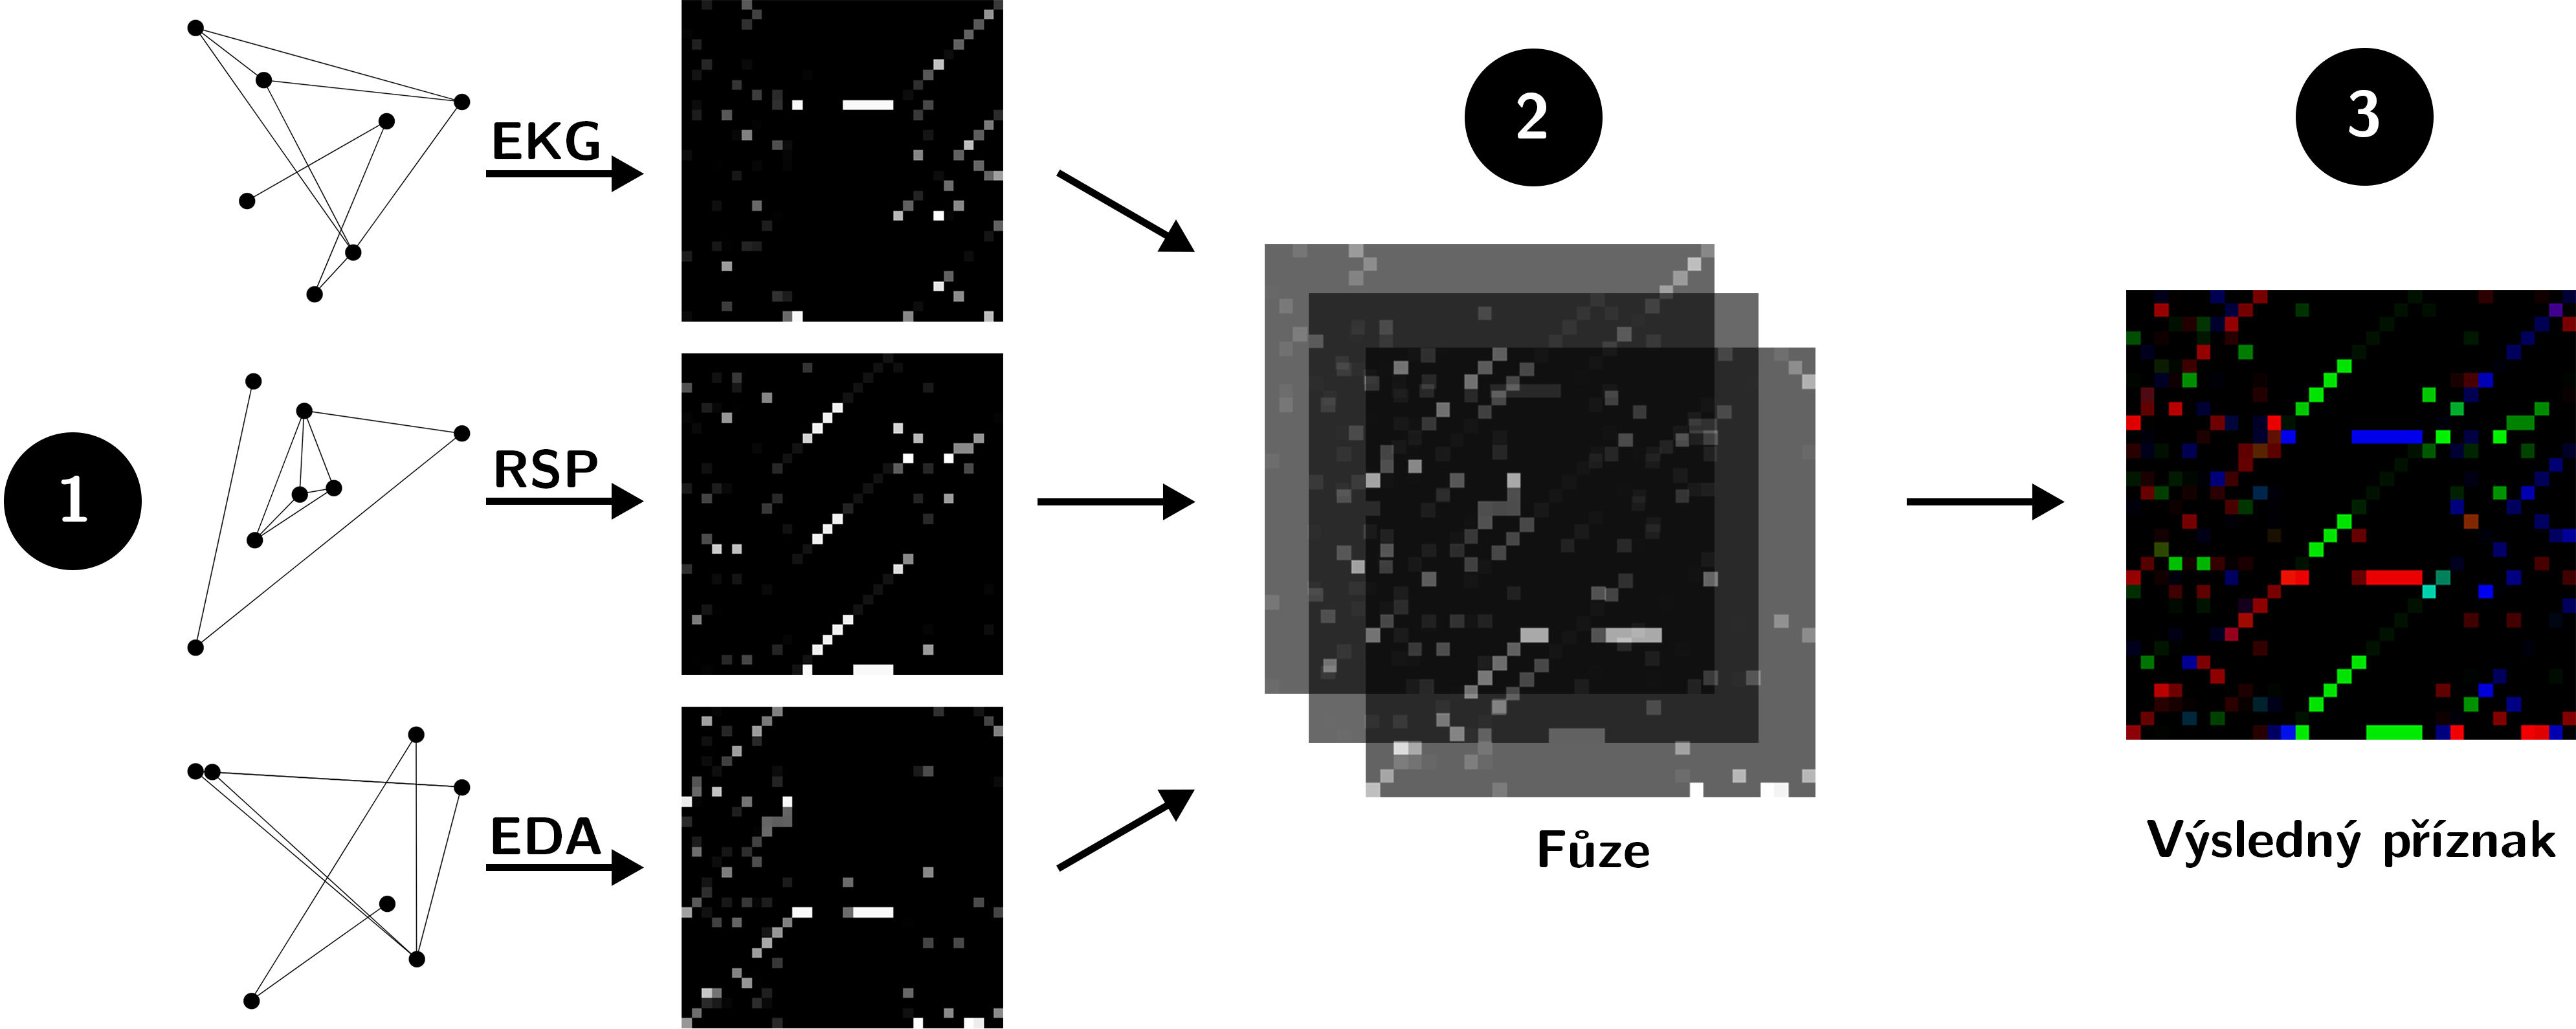
\includegraphics[width=1\linewidth]{figures/GCN}
        \caption{Diagram tvorby kauzálních vícerozměrných matic. 1) Aplikace
            Kopula-Granger metody pro vybraný segment všech kanálů $c$. 2) Kombinace
            výsledných kauzálních matic do jednoho trojrozměrného pole. 3) Výsledný
            příznak ve smyslu RGB obrázku}
        \label{fig:GCN}
    \end{center}
\end{figure}

Kopula-Granger metodu lze primárně shrnout do dvou kroků: odhadnutí marginální
distribuční funkce vybrané časové řady $X^i$ jako $\hat{F_i}$ a mapování
pozorovaných hodnot fyziologické události v čase $t$ do kopula prostoru jako
$Z_{i}^t=\Phi^{-1}\left(\hat{F}_i\left(X_{t}^i\right)\right)$, kde $\Phi$ je
kumulativní distribuční funkce (\gls{CDF}) Gaussova rozdělení. V neposlední řadě
lze konstruovat temporální kauzální graf analýzou relací mezi $Z_{i}^t$. Pro
účely tvorby grafického řešení v podobě kauzální matice $T \times T$ obsahující
odhady koeficientů $\hat{\beta}_i$ byla adaptována regularizovaná regrese
podle~\cite{Bahdori2012}. Nechť vybraná fyziologická událost $X^i = \{x_t^i : t
= 0,...,T\}$, poté lze získat koeficienty následovně:
\begin{equation}
    \hat{\beta}_i(\lambda)=\arg \min _{\beta_i}\left(\sum_{t=1}^T\left\|x_i^t-X_{t, L}^{lag} \beta_i\right\|^2+\lambda\left\|\beta_i\right\|_1\right)
\end{equation}
kde $X_{lag}^{t, L}$ reprezentuje spojený vektor všech zpožděných pozorování s
maximálním zpožděním $L$ až do času $t$. Tvorba kauzálních matic byla
realizována v programovém prostředí Matlab s využitím knihovny
\textit{GLMNET}\footnote{\url{https://hastie.su.domains/glmnet_matlab}}, která
umožňuje specifikovat různé typy regresních modelů. Hodnota časového zpoždění
byla určena na základě Akaikeho informačního kritéria (\gls{AIC}) jako $L = 4$.
Během každého výpočtu bylo pomocí zmíněné knihovny realizováno i automatické
ladění hodnot penalizačního parametru $\lambda \in m_i$, kde $m_i = 10^{a +
(i-1)d}$ pro $i = {1, 2, ..., 6}$ a $d = \frac{b-a}{n-1}$. Hodnoty $a$ a $b$
byly nastaveny na -3 a 2.

\subsection{Konstrukce časoprostorových polí}
\label{subsec:gadf}
Bylo realizováno mapování segmentů všech kanálů $c$ do prostorové domény
(\gls{GAF}), jež zachovává časové závislosti. Wang and Oates~\cite{Wang2015}
představili koncept této metody transformace časové řady do 2D obrazu v roce
2015. Vzhledem k dříve definované fyziologické události, tedy vybrané časové
řadě $X^i = \{x_1^i, x_2^i, \dots, x_t^i\}$ z kanálu $c$ zahrnuje konstrukce
\gls{GAF} nejdříve normalizaci na interval $[-1; 1]$:
\begin{equation}
    \tilde{x}_t=\frac{\left(x_t-\max (X^i)+\left(x_t-\min (X^i)\right)\right.}{\max (X^i)-\min (X^i)}
\end{equation}

\begin{figure}[h]
    \begin{center}
        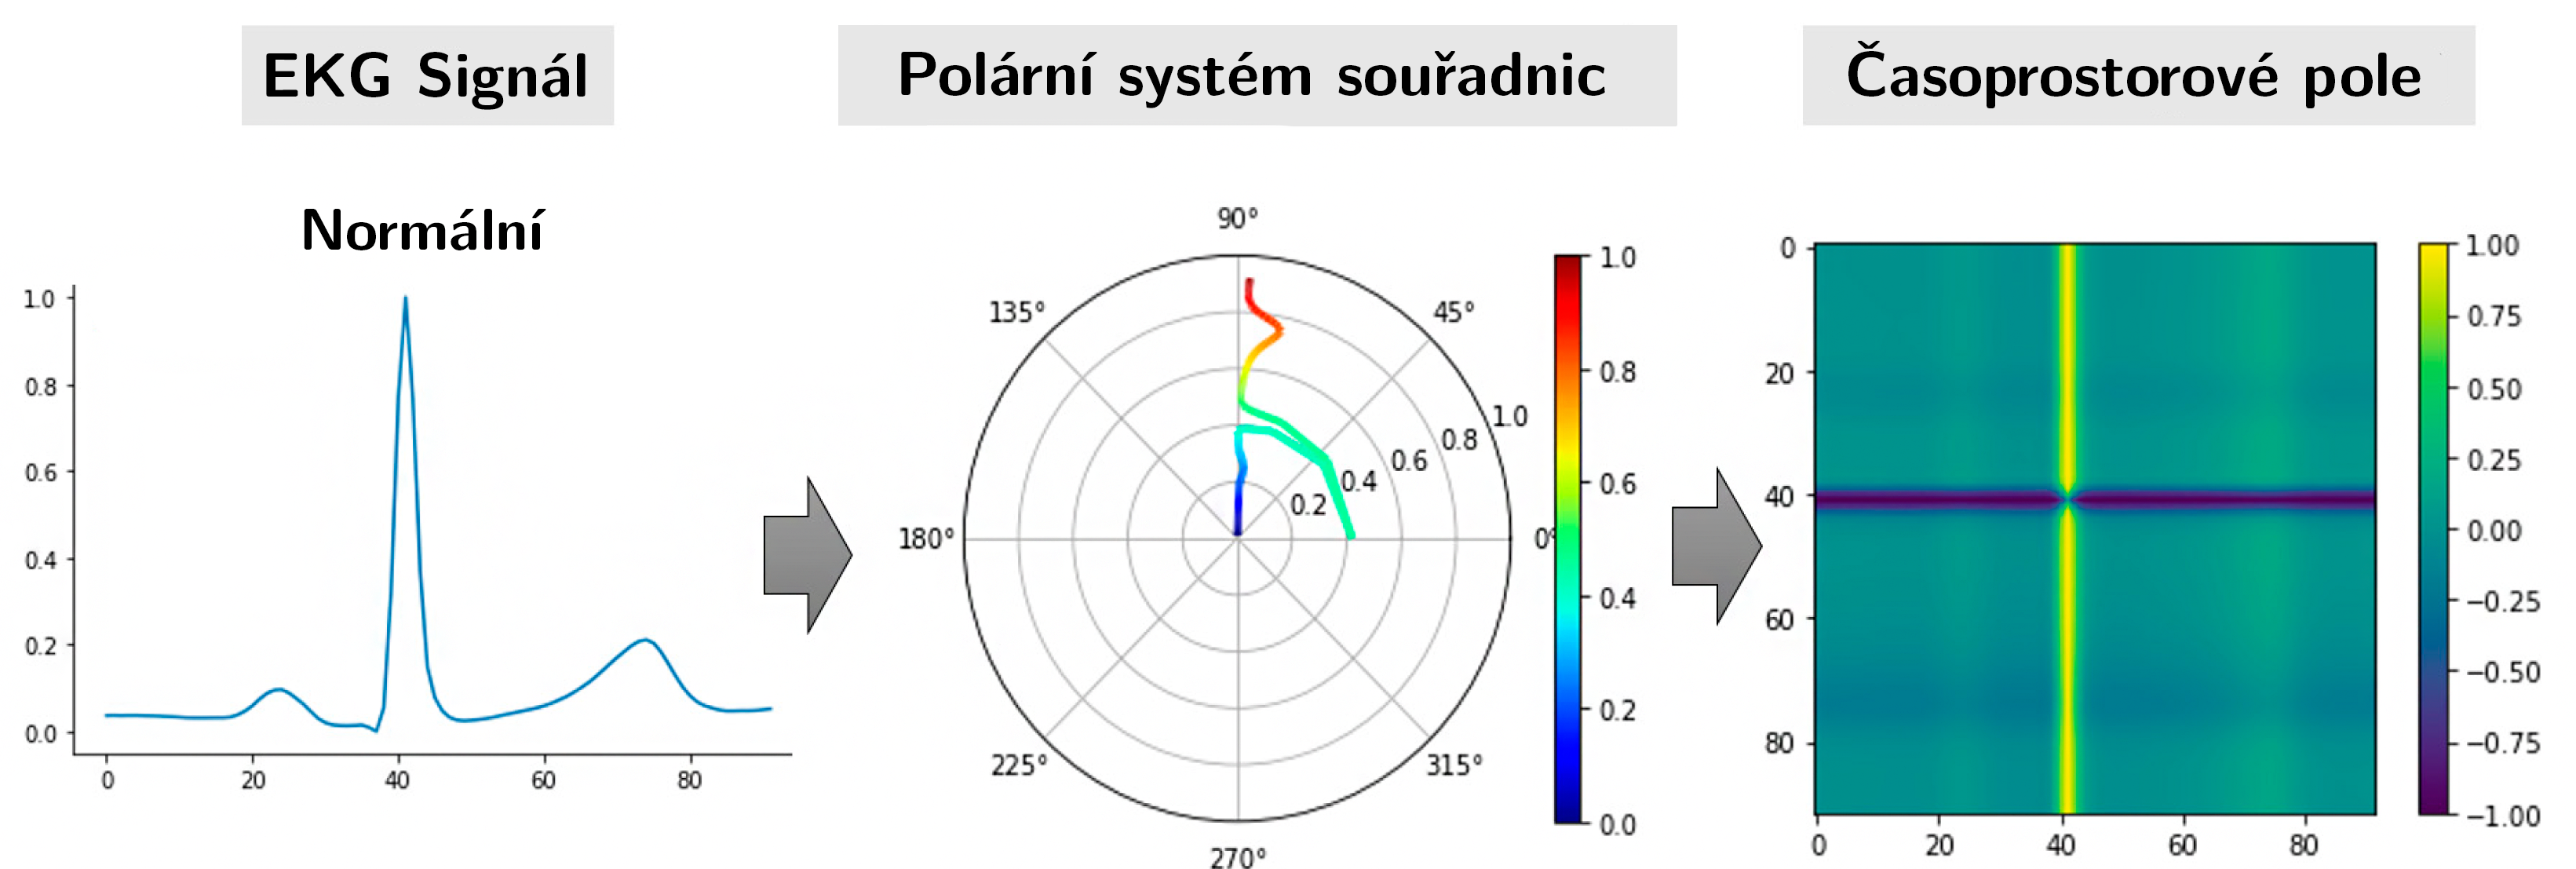
\includegraphics[width=1\linewidth]{figures/polar}
        \caption{Ukázka \gls{GAF} mapování na EKG segmentu~(Upraveno a převzato z~\cite{Zhou2021})}
        \label{fig:polar}
    \end{center}
\end{figure}

Dále jsou normalizovaná data časové řady převedeny do polárních souřadnic
výpočtem úhlové složky $\theta_i$ a radiální složky $r_i$ pro každý vzorek
$\tilde{x}_t$:
\begin{equation}
    \begin{cases}
        \theta_i = \arccos(\tilde{x}_t), & -1 \leq \tilde{x}_t \leq 1, \tilde{x}_t \in \tilde{X^i} \\
        r_i = \frac{t}{N},               & t \in N
    \end{cases}
\end{equation}
kde $t$ je časová značka vzorku fyziologické události a $N$ je konstantní faktor
pro regulaci rozpětí polárního souřadného systému. Jinými slovy, časová značka
představuje poloměr a arkus kosinus hodnoty časové řady úhel. Lze zde hovořit o
bijektivní transformaci, jež zachovává časovou závislost pomocí souřadnice $r$.

Po transformaci přeškálované časové řady do polárního souřadnicového systému lze
využít úhlovou perspektivu, v tomto případě s ohledem na trigonometrický rozdíl
mezi jednotlivými body (\gls{GADF}, Gramian angular field difference), k
identifikaci temporální korelace v rámci různých časových intervalů:
\begin{equation}
    GADF = \left[\sin \left(\phi_i-\phi_j\right)\right]
\end{equation}

\begin{figure}[h]
    \begin{center}
        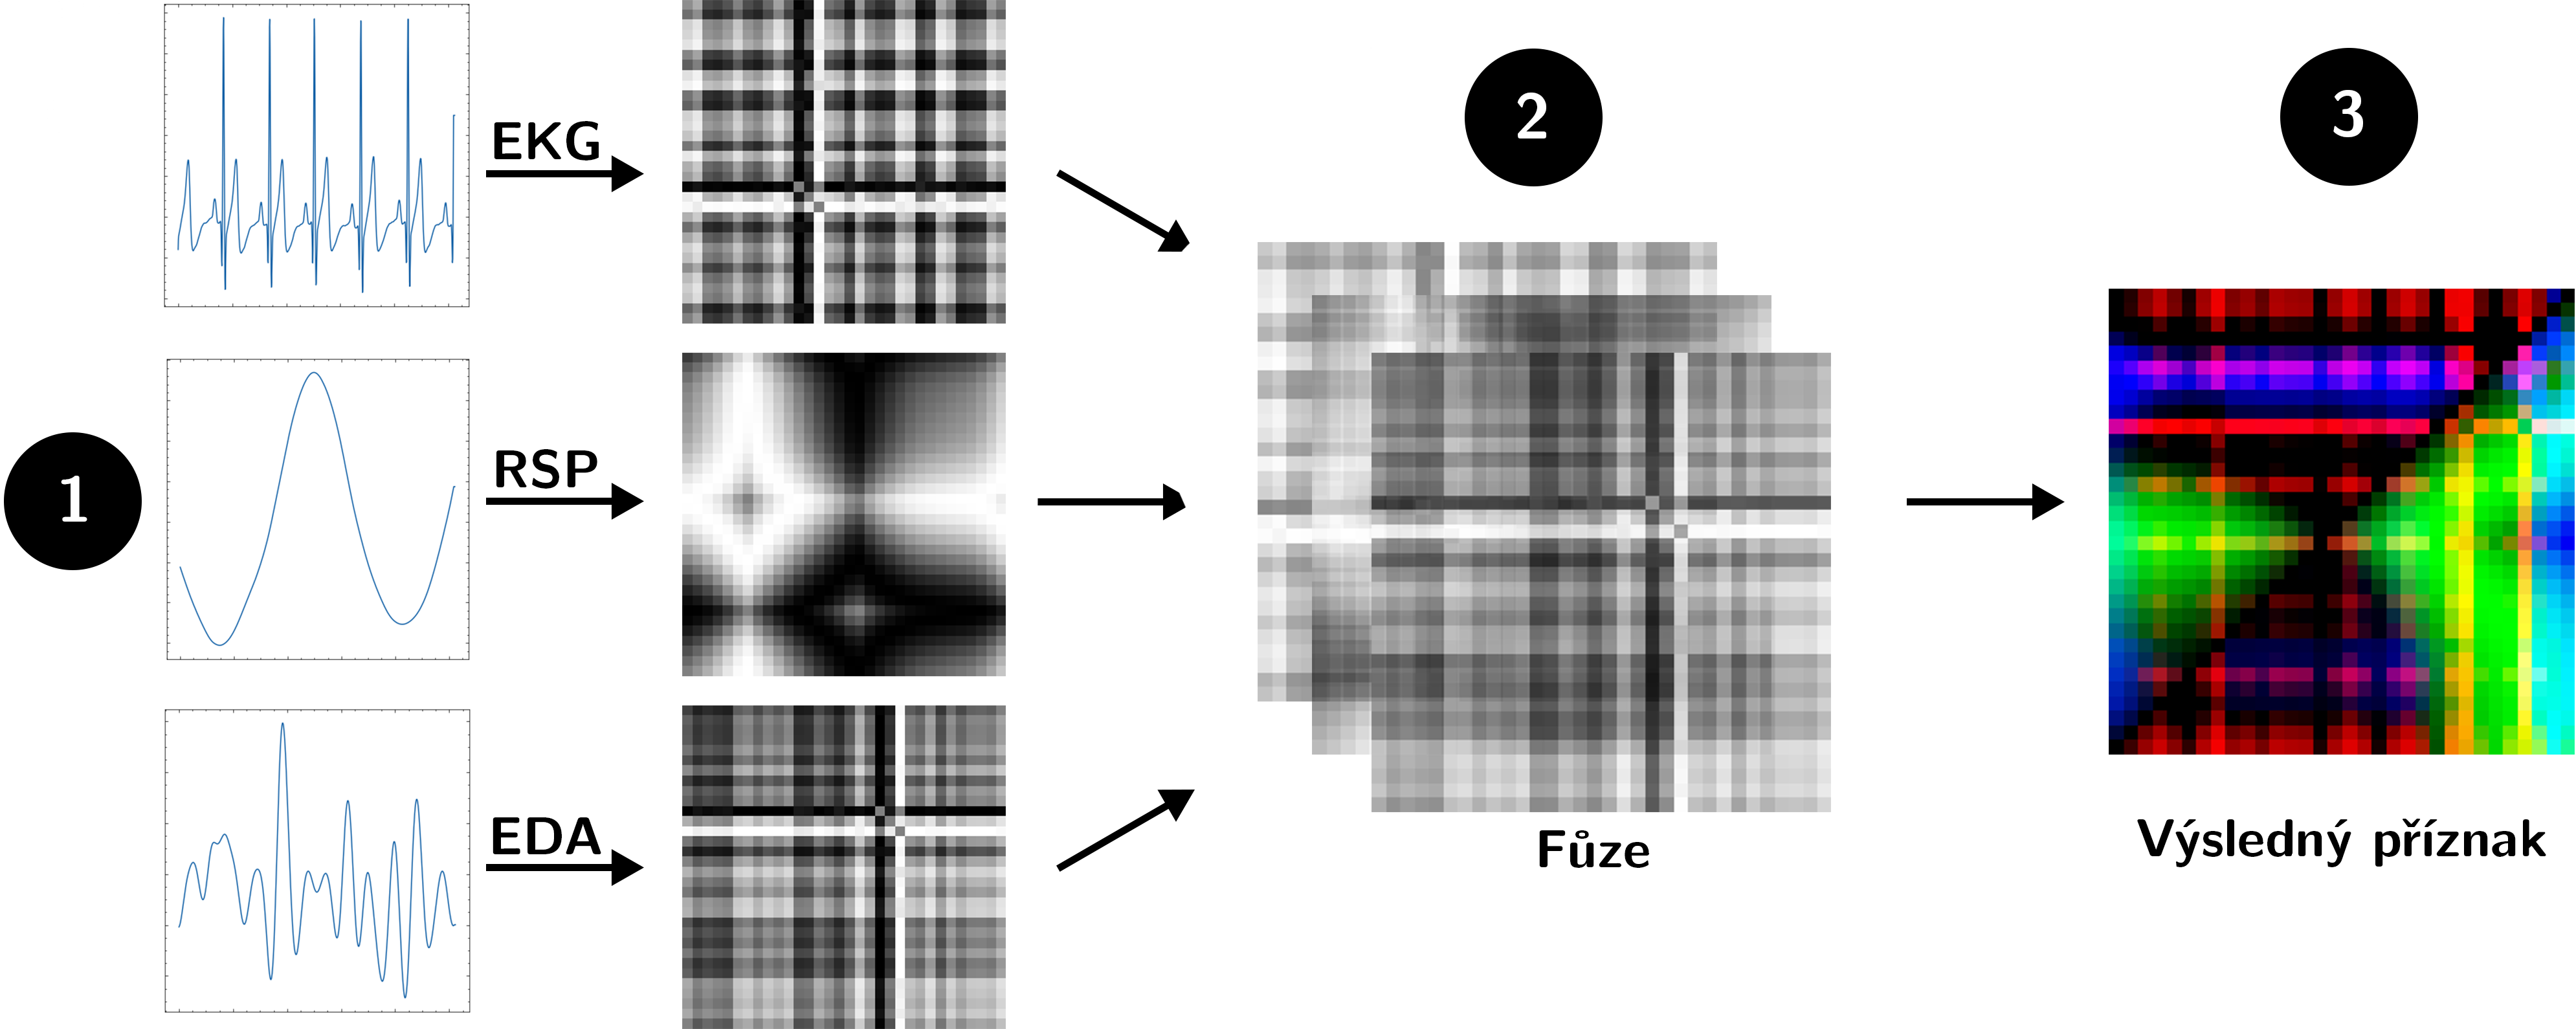
\includegraphics[width=1\linewidth]{figures/GADF}
        \caption{Diagram tvorby časoprostorových vzorů. 1) Aplikace GAF mapování
            pro vybraný segment všech kanálů $c$. 2) Kombinace výsledných polí
            do jednoho trojrozměrného pole. 3) Výsledný příznak kódující
            temporální korelace fyziologické události v prostorové doméně}
        \label{fig:gadf}
    \end{center}
\end{figure}

Ve výsledku je tedy časoprostorový vzor definován následující $T \times T$
maticí, která je kvazi-Gramovou maticí:
\begin{equation}
    GADF = \left[\begin{array}{cccc}
            \sin \left(\phi_1-\phi_1\right) & \sin \left(\phi_1-\phi_2\right) & \cdots & \sin \left(\phi_1-\phi_n\right) \\
            \sin \left(\phi_2-\phi_1\right) & \sin \left(\phi_2-\phi_2\right) & \cdots & \sin \left(\phi_2-\phi_n\right) \\
            \vdots                          & \vdots                          & \ddots & \vdots                          \\
            \sin \left(\phi_n-\phi_1\right) & \sin \left(\phi_n-\phi_2\right) & \cdots & \sin \left(\phi_n-\phi_n\right)
        \end{array}\right]
\end{equation}
kde každý prvek odpovídá sinové funkci úhlového sinusového rozdílu v různých
časových bodech. Výpočet a tvorba těchto příznaků, časoprostorových vzorů, byla
implementována v programovacím jazyce Python.

\subsection{Augmentace dat využitím SMOTENN}
\label{subsec:augmentace_dat}

\subsection{Kapsulární neuronová síť}
\label{subsec:kapsularni_sit}
Pro potřeby realizace úloh klasifikace (resp. hodnocení kognitivní zátěže), byla
navržena architektura kapsulární neuronové sítě postavená na řešení, které
představili Mazzia et al.~\cite{Mazzia2021}, \textit{Efficient-CapsNet}.
Celkovou architekturu lze vidět na obrázku~\ref{fig:architektura}.

\begin{figure}[h]
    \begin{center}
        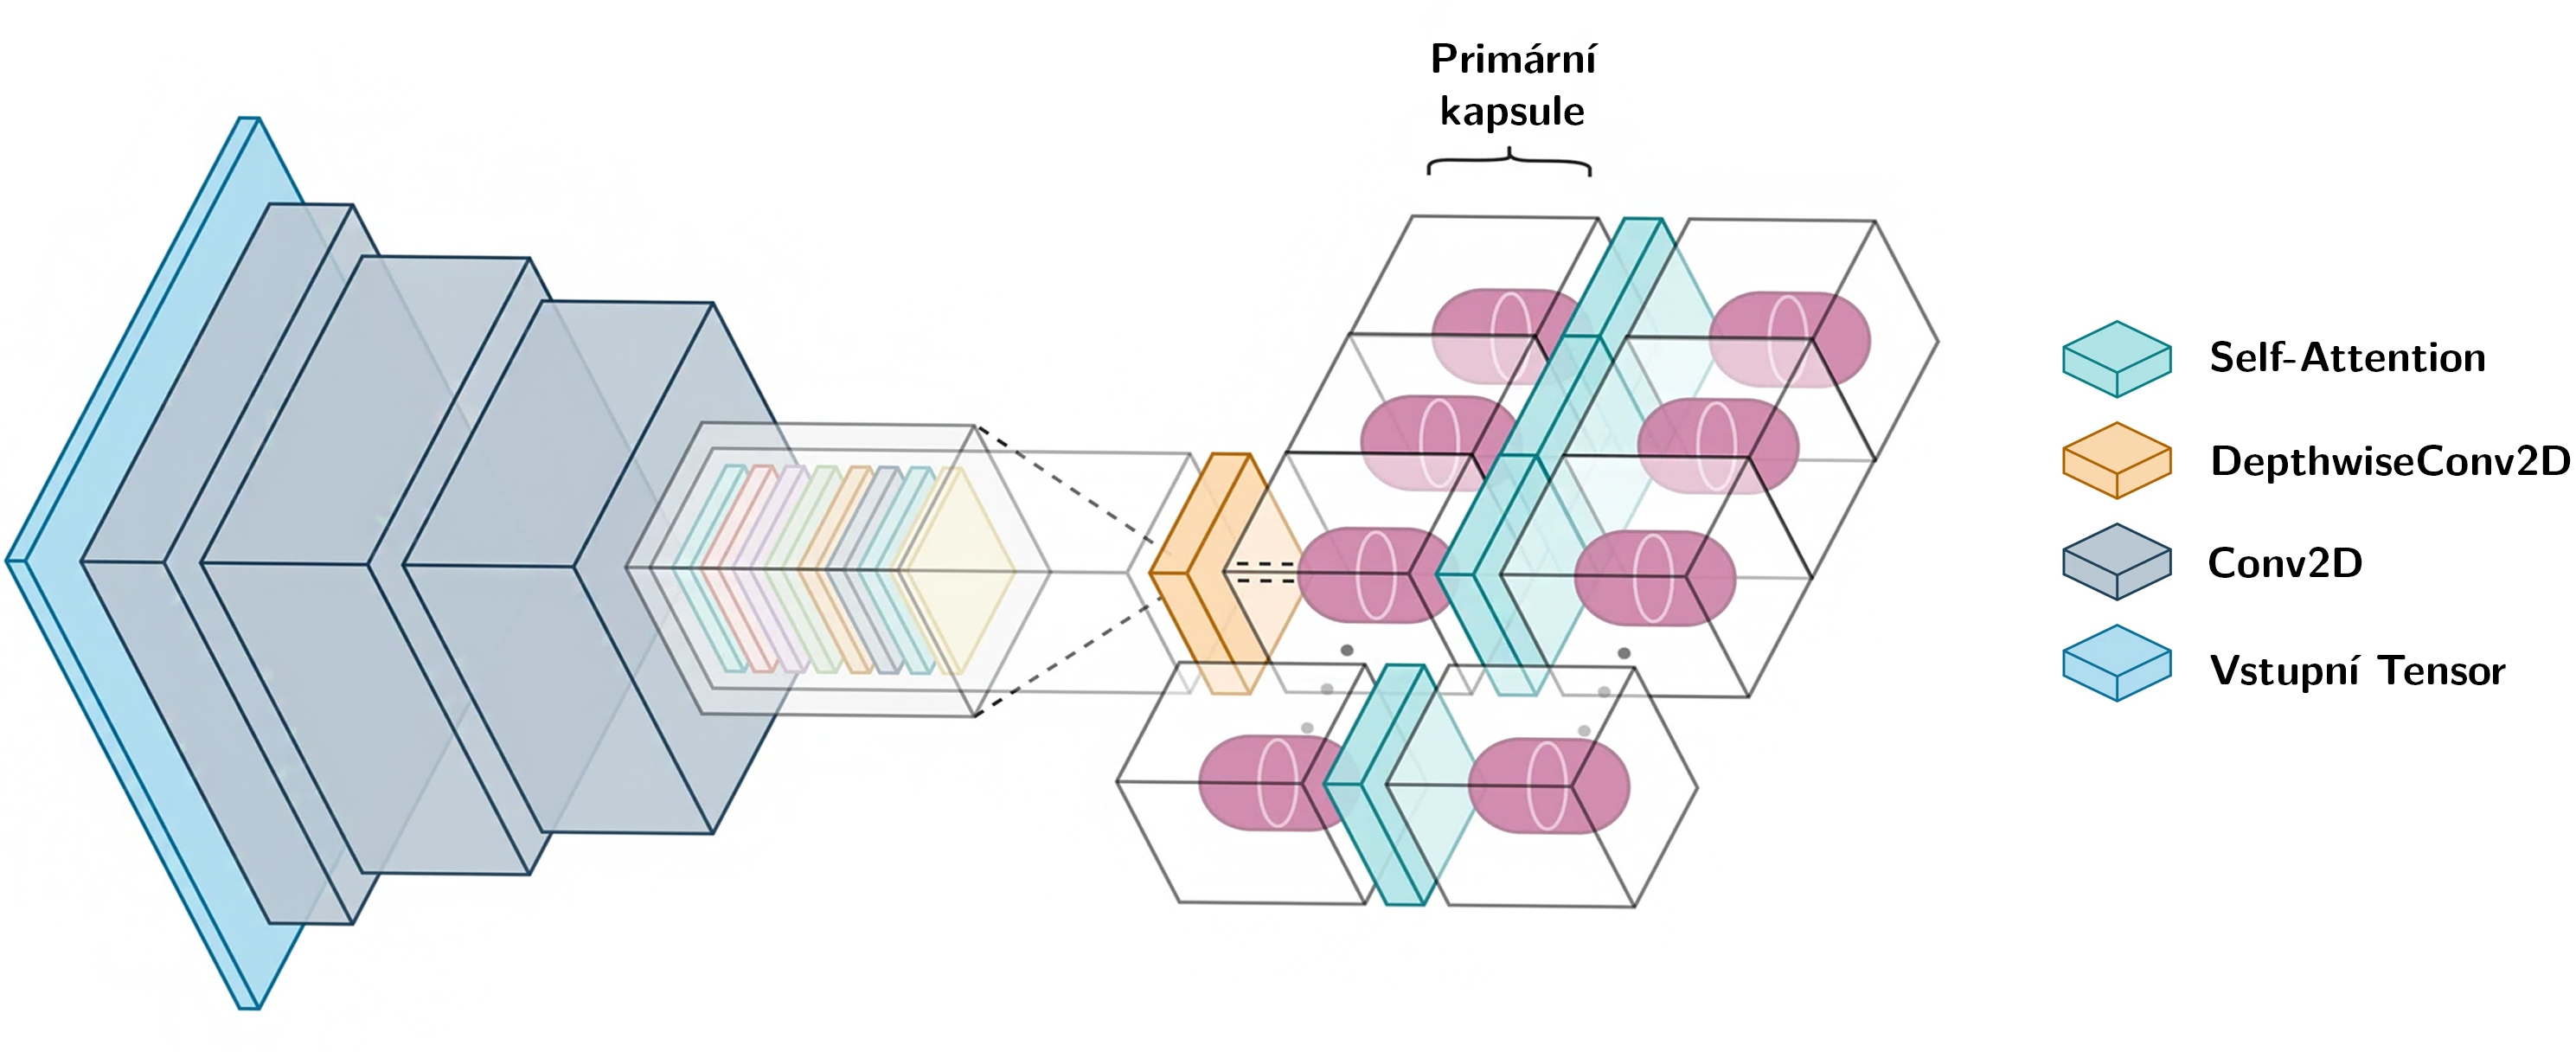
\includegraphics[width=1\linewidth]{figures/capsule}
        \caption{Schematické znázornění architektury sítě
            \textit{Efficient-CapsNet} (Upraveno a převzato z~\cite{Zhou2021})}
        \label{fig:architektura}
    \end{center}
\end{figure}

Zjednodušeně, v případě použití jednoho příznaku, je vstupem modelu obraz, který
lze reprezentovat jako tenzor $X$ s tvarem $H \times W \times C$, kde $H$, $W$ a
$C$ jsou výška, šířka a kanály. V našem případě se jedná o synergické spojení
dvou sad příznaků vyplývajících z minulých sekcí, kauzálních matic $X_{COG} \in
    \mathbb{R}^{T \times T \times C}$ a časoprostorových vzorů $X_{GAF} \in
    \mathbb{R}^{T \times T \times C}$. Vstupním tenzorem je tedy příznak $X \in
    \mathbb{R}^{2 \times T \times T \times C}$. Než se vstup dostane k primární
kapsulové vrstvě, tak je provedena extrakce lokálních vlastnosti ze vstupu $X$
pomocí sady několika typů vrstev\footnote{Jednotlivé vrstvy jsou pojmenovány
    podle korespondujícího názvu v \textit{TensorFlow} a \textit{Keras} API}:
\begin{itemize}
    \item \textbf{Conv2D} --- Tato vrstva vytváří konvoluční jádro, které je
          konvolvováno se vstupem vrstvy a vytváří tenzor výstupů. V podstatě se jedná
          o sadu naučitelných filtrů. Každý filtr transformuje část obrazu
          (definovanou velikostí jádra) pomocí filtru jádra. Matice jádrového filtru
          se aplikuje na celý obraz. Filtry lze chápat jako transformaci obrazu.
    \item \textbf{BatchNormalization} --- Tato vrstva aplikuje normalizaci,
          která udržuje průměrný výstup blízko nule a směrodatnou odchylku výstupu
          blízko jedné.
    \item \textbf{MaxPool2D} --- Tato vrstva funguje jednoduše jako filtr pro
          podvzorkování. Podívá se na 2 sousední pixely a vybere maximální hodnotu.
          Slouží ke snížení výpočetní náročnosti a do jisté míry také ke snížení
          přeučení.
    \item \textbf{Dropout} --- Dropout je regularizační metoda, při níž je část
          uzlů ve vrstvě náhodně ignorována (nastaveny na nulu) pro každý
          tréninkový vzorek. Tím se náhodně vynechá část sítě a síť je nucena
          učit se funkce distribuovaným způsobem. Tato technika také zlepšuje
          generalizaci a snižuje přeučení.
\end{itemize}

\begin{figure}[h]
    \begin{center}
        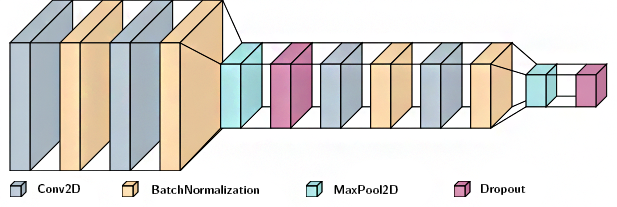
\includegraphics[width=0.85\linewidth]{figures/conv}
        \caption{První část sítě ($H_{Conv}$), která mapuje vstupní obraz na
            prostor vyšší dimenze}
        \label{fig:conv}
    \end{center}
\end{figure}

Každý výstup konvoluční vrstvy $l$ se tedy skládá z konvoluční operace s určitou
rozměrovou velikostí kernelů $k$ a počtem příznakových map $f$. U konvolučních
vrstev byla použita aktivační funkce $\operatorname{ReLU}$ k přidání nelinearity
do sítě:
\begin{equation}
    F^{l+1}\left(X^l\right)=\operatorname{ReLU}\left(\text {Conv}_{k \times k}\left(X^l\right)\right)
\end{equation}
Celkově si lze první část sítě představit jako jednu funkci $H_{Conv}$, která
mapuje vstupní obraz do prostoru s vyšší dimenzí, což usnadňuje tvorbu
kapslí\footnote{\enquote{Kapsle} označuje skupinu neuronů, která společně
představuje instanci parametru specifické entity nebo části obrazu}. Tuto první
část sítě lze vidět na Obr.~\ref{fig:conv}. Následně je pak využito hloubkově
oddělitelné konvoluce, ze které je získána vrstva primárních kapslí $S_{n,d}^l$
kde $n^l$ a $d^l$ jsou počty primárních kapslí a jejich jednotlivé rozměry
$l$-té vrstvy. Základním prvkem sítě tedy již není jeden neuron, ale vektorová
výstupní kapsle, která by měla zachovávat svojí orientaci a délku. To je
realizováno pomocí \enquote{\textit{squash}} aktivační funkce:
\begin{equation}
    \operatorname{squash}\left(s_n^l\right)=\left(1-\frac{1}{e^{\left\|s_n^l\right\|}}\right) \frac{s_n^l}{\left\|s_n^l\right\|}
\end{equation}
kde $s_n^l$ označuje právě jednu kapsli. Detailně koncept kapsulární sítě popsal
Hinton~\cite{Hinton2011}. Kapsulární neuronová síť byla implementována v
programovacím jazyce Python využitím knihoven
\textit{TensorFlow}\footnote{\url{https://www.tensorflow.org}} a
\textit{Keras}\footnote{\url{https://keras.io}}. Počet filtrů konvolučních
vrstev byl zvolen 32, 64, 64 a 128 v pořadí, tak jak jdou za sebou ve
schématu~\ref{fig:conv}. Velikosti kernelů byly zvoleny 5, 3, 3 a 3. MaxPool2D
vrstvy byly přidány k zajištění kombinace lokálních rysů příznaků a učení se tak
jeho globálnějším rysům. 

\subsection{Self-attention směrování}
\label{subsec:dynamicke_smerovani}
Kapsulární síť byla také v této práci zvolena, vzhledem k její architektuře
napodobující lidskou biologii, a tím pádem schopností lépe modelovat komplexní
vztahy v datech. To vyplývá z použitého nového přístupu neiterativního
paralelního směrování kapslí, které bylo představeno a popsáno
v~\cite{Mazzia2021}.

\subsection{Marginální ztrátová funkce}
\label{subsec:marginalni_funkce}
V případě této práce se jedná o binární a vícetřídový klasifikační problém, pro
který by se za normálních okolností použila ztrátová funkce ve smyslu binární
nebo kategorické křížové entropie. Tyto ztrátové funkce ale nezachycují
sémantiku vektorů, jak je používána v kapslích. Pro tyto potřeby byla využita
marginální ztrátová funkce, kde v případě klasifikace více tříd, je pro každou
třídu reprezentovanou kapslí $n^L$ v poslední vrstvě $L$ vypočtena
pravděpodobnost existence určité třídy následovně:
\begin{equation}
    \mathcal{L}_{n^L}=T_{n^L} \max \left(0, m^{+}-\left\|u_n^L\right\|\right)^2+\lambda\left(1-T_{n^L}\right) \max \left(0,\left\|u_n^L\right\|-m^{-}\right)^2
\end{equation}
kde $T_{n^L}$ je rovno jedné, pokud je přítomna třída $n^L$, a $m^+$, $m^-$ a
$\lambda$ jsou laditelné hyperparametry. Nakonec jsou sečteny jednotlivé
ztrátové funkce $\mathcal{L}_{n^L}$ pro získání konečného \enquote{skóre} ve
fázi trénování.

\subsection{Trénování a evaluace modelů}
\label{subsec:trenovani_modelu}

\section{Statistické metody}
\label{sec:statisticke_metody}




% \section{}
% \label{sec:}
% \input{}

% \section{Použité technologie a knihovny}
% \label{sec:technologie_a_knihovny}
% Obory umělé inteligence, jako strojové učení nebo neuronové sítě, často vyžadují
v reálných podmínkách pečlivou přípravu a předzpracování dat nebo sestavení a
trénování modelů. V dnešní době však existuje velké množství nástrojů a
knihoven, které tyto kroky implementují a značně tak zvyšují efektivitu vývoje
patřičných aplikací. Tato kapitola popisuje zásadní nástroje použité pro účely
této práce.

\subsection{Python a R}
\label{subsec:python_r}
Mezi nejpopulárnější open-source programovací jazyky v oblasti strojového učení
a data science, které byly zároveň použity v této práci, patří
Python\footnote{https://www.python.org} a R\footnote{https://www.r-project.org}.
Pro předzpracování dat, strojové učení a neuronové sítě byl použit
Python 3.7 s využitím platformy Google Colab.

Explorační a statistická analýza dat byla realizována prostřednictvím jazyka R
(verze 4.2.1, Funny-Looking Kid) na laptopu \textit{HP Spectre x360} s
procesorem \textit{i7-8705G}, 32~GB DDR4 RAM a grafickou kartou \textit{RX Vega
M GL}. I přestože R není na rozdíl od Pythonu univerzálním vysokoúrovňovým
programovacím jazykem a využívá se především pro statistické modelování, je díky
bohaté komunitě a velkému množství knihoven nedílnou součástí oblasti strojového
učení a data science. 

\subsection{Google Colab a Jupyter Notebook}
\label{subsec:jupyter_colab}
Na základě velkého objemu dat ke zpracování bylo využito platformy Google
Colab\footnote{https://colab.research.google.com}. Jedná se o cloudové
interaktivní výpočetní prostředí, které běží na virtuálním stroji a umožňuje
vzdálené spuštění kódu s využitím prostředků jako \textit{NVIDIA Tesla
V100/P100} s 24~GB VRAM. Jinými slovy jde o hostovanou webovou aplikaci jménem
Jupyter Notebook\footnote{https://jupyter.org}, která umožňuje vytvářet a sdílet
dokumenty (zápisníky). Tyto dokumenty jsou rozděleny do buněk, které lze
spouštět v libovolném pořadí (live kód), což zajišťuje efektivnější
prototypování.

\subsection{Neurokit}
\label{subsec:neurokit}
Knihovna Neurokit2~\cite{Makowski2021neurokit} poskytuje pokročilé metody pro
zpracování a vizualizaci biosignálu. Jednotlivé metody zároveň nabízejí možnost
si vybrat z mnoha implementovaných algoritmů, například pro detekci QRS
komplexu. V této práci byla knihovna použita pro předzpracování respirační,
elektrodermální a srdeční aktivity včetně zpracování HRV.

\subsection{Tidyverse a Easystats}
\label{subsec:tidyverse_easystats}
Knihovny tidyverse~\cite{tidyverse} a easystats~\cite{easystats} rozšiřují jazyk
R o mnoho funkcionalit primárně pro potřeby statistického modelování a
strojového učení. Usnadňují a zrychlují proces tvorby modelů díky dobře
zdokumentovanému ekosystému balíčků. V této práci sloužili knihovny ke
statistické analýze velkého souboru dat. 

\subsection{Scikit-learn, TensorFlow a Keras}
\label{subsec:scitkit_tensor_keras}
Scikit-learn~\cite{sklearn_api} je balíček jazyka Python pro prediktivní analýzu
dat a strojové učení, který byl v této práci použit pro extrakci a normalizaci
příznaků. Dále pro porovnávání, validaci a výběr parametrů a modelů.

% TensorFlow is an open-source framework developed at Google for machine learning
% applications. Its main focus is on defining the architecture and training of
% deep neural networks. It is highly optimized for the execution of low level
% tensor operations on CPU, GPU, or TPU. 

% Keras is a high-level API that acts as an interface for the TensorFlow
% framework. It enables faster prototyping of ANNs by providing abstractions and
% building blocks for developing the models. It also provides the implementation
% of several popular CNN architectures along with their weights, making transfer
% learning more accessible. The simplest way of defining Keras models is by using
% the Sequential model API, which is essentially a linear stack of defined layers.
% The alternative is adopting the Keras functional API, which allows for building
% arbitrary graphs of layers with multiple inputs and outputs or using residual
% skipping connections.

\subsection{InfluxDB}
\label{subsec:influx}
InfluxDB\footnote{https://www.influxdata.com} je open-source platforma
poskytující databázi pro časové řady. Zahrnuje rozhraní (API) pro standardní
databázové dotazy. Součástí je i grafické uživatelské rozhraní (GUI) s
modulárními uživatelskými panely pro monitorování dat v reálném čase. Tato
platforma (InfluxDB OSS 2.4) byla využita v rámci experimentální části práce k
uchovávání a vizualizaci dat.



% \section{Statistické metody}
% \label{sec:_statisticke_metody}
% 



% \begin{figure}[ht]
%     \centering
%     \begin{subfigure}[b]{0.45\textwidth}
%       \mybox{dirs}{%
%       \dirtree{%
%       .1 COVIDx8B.
%       .2 labels.
%       .3 train\_COVIDx8B.txt.
%       .3 test\_COVIDx8B.txt.
%       .2 train.
%       .3 Image\_1.
%       .3 Image\_2.
%       .3 \vdots.
%       .2 test.
%       .3 Image\_1.
%       .3 Image\_2.
%       .3 \vdots.
%       }
%       \tcblower
%       \caption{Original COVIDx8B}
%       \label{subfig:tree1}
%       }
%     \end{subfigure}
%     \begin{subfigure}[b]{0.45\textwidth}
%       \mybox{dirs}{%
%       \dirtree{%
%       .1 COVIDx8B.
%       .2 train.
%       .3 negative.
%       .4 Image\_1.
%       .4 Image\_2.
%       .4 \vdots.
%       .3 positive.
%       .4 Image\_1.
%       .4 Image\_2.
%       .4 \vdots.
%       .2 test.
%       .3 negative.
%       .4 Image\_1.
%       .4 Image\_2.
%       .4 \vdots.
%       .3 positive.
%       .4 Image\_1.
%       .4 Image\_2.
%       .4 \vdots.
%       }
%       \tcblower
%       \caption{Preprocessed COVIDx8B}
%       \label{subfig:tree2}
%       }
%     \end{subfigure}
%     \caption[Comparison of the directory tree of the original COVIDx8B dataset and our preprocessed version]{Comparison of the directory tree of the original COVIDx8B dataset (a) as used by the COVID-Net project, and the preprocessed version (b) which was used in our experiments for image generation during training.}
%     \label{fig:directory_comparison}
%   \end{figure}